\documentclass{cmspaper}
\usepackage{epsfig}
\usepackage{epstopdf}
\usepackage[usenames]{color}
\usepackage{multirow}
\usepackage{amsmath}
\usepackage{amssymb}
%\usepackage{here}
\usepackage{shortvrb,rotating}
\usepackage{subfigure}
% Roerto macros
\newcommand{\qu}{u}
\newcommand{\qd}{d}
\newcommand{\qubar}{\bar u}
\newcommand{\qdbar}{\bar d}
\newcommand{\bfig}{\begin{center}\begin{picture}}
\newcommand{\efig}[1]{\end{picture}\\{\small #1}\end{center}}
\newcommand{\flin}[2]{\ArrowLine(#1)(#2)}
\newcommand{\wlin}[2]{\DashLine(#1)(#2){2.5}}
\newcommand{\zlin}[2]{\DashLine(#1)(#2){5}}
\newcommand{\glin}[3]{\Photon(#1)(#2){2}{#3}}
\newcommand{\lin}[2]{\Line(#1)(#2)}
\newcommand{\noi}{\noindent}
\newcommand{\sof}{\SetOffset}
\newcommand{\bmip}[2]{\begin{minipage}[t]{#1pt}\bfig(#1,#2)}
\newcommand{\emip}[1]{\efig{#1}\end{minipage}}
\newcommand{\putk}[2]{\Text(#1)[r]{$p_{#2}$}}
\newcommand{\putp}[2]{\Text(#1)[l]{$p_{#2}$}}
\newcommand{\bq}{\begin{equation}}
\newcommand{\eq}{\end{equation}}
\newcommand{\bqa}{\begin{eqnarray}}\newcommand{\eqa}{\end{eqnarray}}
\newcommand{\nl}{\nonumber \\}
\newcommand{\eqn}[1]{Eq. (\ref{#1})}
\newcommand{\eqs}[1]{eqs. (\ref{#1})}
\newcommand{\ibidem}{{\it ibidem\/},}
\newcommand{\vpb}{}
\newcommand{\p}[1]{{\scriptstyle{\,(#1)}}}
\newcommand{\gev}{\mbox{GeV}}
\newcommand{\tev}{\mbox{TeV}}
\newcommand{\mev}{\mbox{MeV}}
\setcounter{section}{0}
\setcounter{subsection}{0}
\setcounter{paragraph}{0}
\setcounter{subparagraph}{0}
\setcounter{equation}{0}
\setcounter{figure}{0}
\setcounter{table}{0}
\setcounter{footnote}{0}
\setcounter{mpfootnote}{0}
% MLM's macros
\def    \eqnum          #1{(\ref{#1})}       %equation # in round parenthesis
\def    \scite          #1{$^{\cite{#1}}$}     %superscript biblio ref

  \newcommand{\ccaption}[2]{
    \begin{center}
    \parbox{0.85\textwidth}{
      \caption[#1]{\small{{#2}}}
      }
    \end{center}
    }
\newcommand{\BS}{\bigskip}
% MATH SYMBOLS
\def    \be             {\begin{equation}}
\def    \ee             {\end{equation}}
\def    \ba             {\begin{eqnarray}}
\def    \ea             {\end{eqnarray}}
\def    \nn             {\nonumber}
\def    \=              {\;=\;}
\def    \frac           #1#2{{#1 \over #2}}
\def    \ret            {\\[\eqskip]}
\def    \ie             {{\em i.e.\/} }
\def    \eg             {{\em e.g.\/} }
\def   \apr       {{\em a priori} }
\def   \apo      {{\em a posteriori} }
%\def \lsim{\mathrel{\vcenter
%     {\hbox{$<$}\nointerlineskip\hbox{$\sim$}}}}
%\def \gtrsim{\mathrel{\vcenter
%     {\hbox{$>$}\nointerlineskip\hbox{$\sim$}}}}
\def    \bentarrow      {\:\raisebox{1.1ex}{\rlap{$\vert$}}\!\rightarrow}
\def    \rd             {{\mathrm d}}    
\def    \Im             {{\mathrm{Im}}}  
\def    \bra#1          {\mbox{$\langle #1 |$}}
\def    \ket#1          {\mbox{$| #1 \rangle$}}

% UNITS                 
\def    \kev            {\mbox{$\mathrm{keV}$}}
\def    \mev            {\mbox{$\mathrm{MeV}$}}
\def    \gev            {\mbox{$\mathrm{GeV}$}}

% PARTICLE SYMBOLS
\def    \nubar   {\bar{\nu}}
\def    \ubar   {\bar{u}}
\def    \dbar   {\bar{d}}
\def    \qbar   {\bar{q}}
\def    \bbar   {\bar{b}}
\def    \cbar   {\bar{c}}
\def    \cpbar   {\bar{c}'}
\def    \tbar   {\bar{t}}
\def    \Qbar   {\overline{Q}}

% KINEMATICAL VARIABLES 
\def    \mq             {\mbox{$m_Q$}}  
\def    \mZ             {\mbox{$m_Z$} }
\def    \mZsq             {\mbox{$m_Z^2$} }
\def    \mW             {\mbox{$m_W$} }
\def    \mWsq             {\mbox{$m_W^2$} }
\def    \mH             {\mbox{$m_H$} }
\def    \mHsq             {\mbox{$m_H^2$} }
\def    \mt             {\mbox{$m_t$}}  
\def    \mtsq             {\mbox{$m_t^2$}}  
\def    \mb             {\mbox{$m_b$}}  
\def    \mbsq             {\mbox{$m_b^2$}}  
\def    \mqq            {\mbox{$m_{Q\bar Q}$}}
\def    \mqqsq          {\mbox{$m^2_{Q\bar Q}$}}
\def    \pt             {\mbox{$p_T$}}
\def    \et             {\mbox{$E_T$}}
\def    \xt             {\mbox{$x_T$}}
\def    \xtsq           {\mbox{$x_T^2$}}
\def    \ptsq           {\mbox{$p^2_T$}}
\def    \ptbsq           {\mbox{$p^2_{T,b}$}}
\def    \ptbbsq           {\mbox{$p^2_{T,\bar{b}}$}}
\def    \ptWsq           {\mbox{$p^2_{T,W}$}}
\def    \ptZsq           {\mbox{$p^2_{T,Z}$}}
\def    \mT             {\mbox{$m_T$}}
\def    \mTsq           {\mbox{$m^2_T$}}
\def    \etsq           {\mbox{$E^2_T$}}
        
% QCD PARAMETERS                                      
\newcommand     \MSB            {\ifmmode {\overline{\rm MS}} \else 
                                 $\overline{\rm MS}$  \fi}
\def    \muf            {\mbox{$\mu_{\rm F}$}}
\def    \mug            {\mbox{$\mu_\gamma$}}
\def    \mufsq          {\mbox{$\mu^2_{\rm F}$}}
\def    \mur            {{\mbox{$\mu_{\rm R}$}}}
\def    \mursq          {\mbox{$\mu^2_{\rm R}$}}
\def    \mul            {{\mu_\Lambda}}
\def    \mulsq          {\mbox{$\mu^2_\Lambda$}}

\def    \bzero          {\mbox{$b_0$}}
\def    \as             {\ifmmode \alpha_s \else $\alpha_s$ \fi}
\def    \aem             {\mbox{$\alpha_{em}(\mZ)$}}
\def    \asb            {\mbox{$\alpha_s^{(b)}$}}
\def    \assq           {\mbox{$\alpha_s^2$}}
\def \oacube {\mbox{$ {\cal O}(\alpha_s^3)$}}
\def \oaemacube {\mbox{$ {\cal O}(\alpha\alpha_s^3)$}}
\def \oafour {\mbox{$ {\cal O} (\alpha_s^4)$}}
\def \oatwo {\mbox{$ {\cal O} (\alpha_s^2)$}}
\def \oaematwo {\mbox{$ {\cal O}(\alpha \alpha_s^2)$}}
\def \oaemas {\mbox{$ {\cal O}(\alpha \alpha_s)$}} 
\def \oas   {\mbox{$ {\cal O}(\alpha_s)$}}
\def\slash#1{{#1\!\!\!/}}
\def\rt1{\raisebox{-1ex}{\rlap{$\; \rho \to 1 \;\;$}}
\raisebox{.4ex}{$\;\; \;\;\simeq \;\;\;\;$}}
\def\ltap{\raisebox{-.5ex}{\rlap{$\,\sim\,$}} \raisebox{.5ex}{$\,<\,$}}
\def\gtap{\raisebox{-.5ex}{\rlap{$\,\sim\,$}} \raisebox{.5ex}{$\,>\,$}} 

\newcommand\LambdaQCD{\Lambda_{\scriptscriptstyle \rm QCD}}
\def\naive{na\"{\i}ve}
\def\asp{{\alpha_s}\over{\pi}}
\def\half{\frac{1}{2}}
\def\herwig{{\small HERWIG}}
\def\isajet{{\small ISAJET}}
\def\pythia{{\small PYTHIA}}
\def\grace{{\small GRACE}}
\def\amegic{{\small AMEGIC++}}
\def\vecbos{{\small VECBOS}}
\def\madgraph{{\small MADGRAPH}}
\def\comphep{{\small CompHEP}}
\def\ALPHA{{\small ALPHA}}
\def\ALPGEN{{\small ALPGEN}}
\def\SHERPA{{\small SHERPA}}
\def\ppbar{\mbox{$p \bar{p}$}}
\def\met{$\rlap{\kern.2em/}E_T$}
%%%%%%%%%%%%%%%%%%%%%%%%%%%%%%%%%%%%%%%%%%%%%%%%%%%%%%%%%%%%%%%%%%%%%%

\begin{document}
%\MakeShortVerb{\|}
%%%%%%%%%%%%%%%%%%%%%%%% DEFINITIONS
\renewcommand{\arraystretch}{1.7}
%%%%%%%%%%%%%%%%%%%%%%%% TITLE PAGE
%==============================================================================
% title page for few authors

\begin{titlepage}
\analysisnote{2009/XXX} 
\today ~{\bf DRAFT}
\boldmath \title{
Particle Flow Jet Composition
} \unboldmath
\begin{Authlist}
Francesco Pandolfi, Daniele del Re
%
\begin{center}
 \begin{small}
%$^a$ {\it CERN, European Organization for Nuclear Research, Geneva, Switzerland} \\
%$^b$ {\it California Institute of Technology, Pasadena, California, U.S.A.} \\ 
%$^c$ {\it Universit\'{a} di Pisa e Sezione dell' INFN, Roma, Italy} \\
%$^d$ {\it Fermi National Accelerator Laboratory (FNAL)} \\
 {\it ``Sapienza'' Universit\`{a} di Roma e Sezione dell'INFN, Roma, Italy} \\
%$^f${\it Instituto de Fisica Teorica-Universidade Estadual Paulista, Sao Paulo, Brazil} \\
%$^g$ {\it Ghent University, Ghent, Belgium} \\
\end{small}
\end{center}
\end{Authlist}
% Authorlist:
% Primary authors 
% will be those who thought and worked on the topic significanlty and wrote
% the note; the rest of the team that assisted with comments,improvements,
% oversight
% and remarks etc in meetings will go always
% as co-author. \\ co-author theorists if any\\
% to qualify as a primary author one (or more)
% of the following needs to be true
% 1. Was this work initiated by me?
% 2. Did I do most of the work to produce the results of this note?
% 3. Did I write most of this note?
% 4. Did I have a breakthrough idea  that raised the knowledge and scientific value of this note?
% If you answer yes to any of this you are a primary author
%
% If there are less than 4 primary authors they go by seniority starting from the students;
% If there are more than 4 primary authors
% there are two options:
%  put them also in alphabetical order  (prefered for the ratio notes e.g.
% where even if we split them there is more than 4 authors)
%% Note  since these are not CMS public documents the
%% authorlist ordering is for motivation and reward within the
%% working team.
\begin{abstract}
sblearch.
\end{abstract} 
\end{titlepage}
\tableofcontents
\newpage


\section{Introduction}

The Particle Flow event reconstruction \cite{pflow} aims at giving a complete description of the event by reconstructing all final state stable particles. In order to do this, all CMS sub-detectors are exploited in unison in an optimal way. Reconstructed particle candidates are then grouped together to form Particle Flow jets.

The Particle Flow substantially improves jet reconstruction in CMS, delivering jets that are measured more accurately than the ones provided by calorimeter-based reconstruction algorithms. This phenomenon is amplified at low $p_{\mathrm{T}}$, and is due to three main reasons:
\begin{itemize}
\item the Particle Flow algorithm is constructed in such a way that at low $p_{\mathrm{T}}$ it makes more extensive relying on the very precise track information; calorimeter jets, conversely, are very inaccurate at low energies, with their resolution dominated by the fluctuations induced by the noise and stochastic HCAL terms;
\item soft charged jet particles are bent away by the 3.8 T magnetic field, and therefore create deposits far away in the calorimeter with respect to the jet axis; these particles can be recovered by making use of the tracker information, whereas in a calorimeter stand-alone approach they are invariably lost;
\item the superior tracker granularity allows a correct inter-particle momentum subdivision even for collimated bunches of particles, resulting in a more accurate evaluation of the jet 4-vector.
\end{itemize}

Compared to traditional jet reconstruction, though, a Particle Flow jet is a more complex object. Therefore, more detailed analyses can and must be done in order to monitor and improve their performance.

This note describes one of such methods, based on the study of a Particle Flow jet's particle composition. Different jet sub-populations can be defined, depending on what fraction of its energy is carried by a certain type of particles. Studying the jet qualities as a function of the variations of these energy fractions gives powerful insight on the nature of the jet itself. One of these variables, the fraction of jet energy carried by charged hadron candidates, proves to be a valid meter of the quality with which the jet has been reconstructed. It can therefore be exploited at analysis level, to select Particle Flow jets that have been measured more accurately, or as a calibration variable, to optimally take into account different classes of jet sub-populations.


\begin{table}[b]
\belowcaptionskip 0cm
\caption{Analyzed `Summer 09' QCD di-jet samples. For each sample, its DBS instance, cross section ($\sigma$), and number of events is given.}
\label{tab:dbs_dijet}
\begin{center}
\renewcommand{\baselinestretch}{0.8}
\small\normalsize
\begin{tabular}{lcc}
\hline
{\bf DBS Instance}& {\bf $\sigma$ [pb] } & {\bf Events} \\ 
\hline 
/QCDDiJetPt0to15/Summer09-MC\_31X\_V3-v1/GEN-SIM-RECO & $5.16\cdot 10^{10}$ & 2516828 \\
/QCDDiJetPt15to20/Summer09-MC\_31X\_V3-v1/GEN-SIM-RECO & 9.49$\cdot 10^8$ & 2018990 \\
/QCDDiJetPt20to30/Summer09-MC\_31X\_V3-v1/GEN-SIM-RECO & 4.01$\cdot 10^8$ & 1696590\\
/QCDDiJetPt30to50/Summer09-MC\_31X\_V3-v1/GEN-SIM-RECO & 9.47$\cdot 10^7$ & 1094811\\
/QCDDiJetPt50to80/Summer09-MC\_31X\_V3-v1/GEN-SIM-RECO & 1.22$\cdot 10^7$ & 119642\\
/QCDDiJetPt80to120/Summer09-MC\_31X\_V3-v1/GEN-SIM-RECO & 1.62$\cdot 10^6$ & 551544\\
/QCDDiJetPt120to170/Summer09-MC\_31X\_V3-v1/GEN-SIM-RECO & 2.56$\cdot 10^5$ & 54568\\
/QCDDiJetPt170to230/Summer09-MC\_31X\_V3-v1/GEN-SIM-RECO & 4.83$\cdot 10^4$ & 55000\\
/QCDDiJetPt230to300/Summer09-MC\_31X\_V3-v1/GEN-SIM-RECO & 1.06$\cdot 10^4$ & 54028\\
/QCDDiJetPt300to380/Summer09-MC\_31X\_V3-v1/GEN-SIM-RECO & 2.63$\cdot 10^3$ & 52356\\
/QCDDiJetPt380to470/Summer09-MC\_31X\_V3-v1/GEN-SIM-RECO & 7.22$\cdot 10^2$ & 54559\\
/QCDDiJetPt470to600/Summer09-MC\_31X\_V3-v1/GEN-SIM-RECO & 2.41$\cdot 10^2$ & 55905\\
/QCDDiJetPt600to800/Summer09-MC\_31X\_V3-v1/GEN-SIM-RECO & 6.25$\cdot 10^1$ & 21424\\
/QCDDiJetPt800to1000/Summer09-MC\_31X\_V3-v1/GEN-SIM-RECO & 9.42 & 21028\\
/QCDDiJetPt1000to1400/Summer09-MC\_31X\_V3-v1/GEN-SIM-RECO & 2.34 & 21784\\
/QCDDiJetPt1400to1800/Summer09-MC\_31X\_V3-v1/GEN-SIM-RECO & 1.57$\cdot 10^{-1}$ & 21810\\
/QCDDiJetPt1800to2200/Summer09-MC\_31X\_V3-v1/GEN-SIM-RECO & 1.38$\cdot 10^{-2}$ & 21730\\
/QCDDiJetPt2200to2600/Summer09-MC\_31X\_V3-v1/GEN-SIM-RECO & 1.30$\cdot 10^{-3}$ & 22013\\
/QCDDiJetPt2600to3000/Summer09-MC\_31X\_V3-v1/GEN-SIM-RECO & 1.14$\cdot 10^{-4}$ & 22046\\
/QCDDiJetPt3000to3500/Summer09-MC\_31X\_V3-v1/GEN-SIM-RECO & 8.43$\cdot 10^{-6}$ & 20908\\
/QCDDiJetPt3500toInf/Summer09-MC\_31X\_V3-v1/GEN-SIM-RECO & 1.81$\cdot 10^{-7}$ & 21060\\
\hline
\end{tabular}
\end{center}
\end{table}
\section{Data Samples}

This analysis makes use of two different sets of data samples from the `Summer 09' production. These events have all been generated and reconstructed with the {\tt CMSSW\_3\_1\_X} software release series, at a centre of mass energy $\sqrt{s} = 10$ TeV. The analysis has been made entirely in {\tt CMSSW\_3\_1\_2}.

The results presented in Sections \ref{sec:composition} and \ref{sec:MCtest} have been obtained by analyzing the  QCD di-jet samples, which have been generated in 21 parton transverse momentum ($\hat{p}_{\mathrm{T}}$) bins. The DBS instances of these datasets, as well as the corresponding cross sections and number of events, are shown in Table \ref{tab:dbs_dijet}. On the other hand, the data-driven method for computing and applying such corrections, described in Section \ref{sec:photJet}, makes use of the Photon+Jet samples, listed in Table \ref{tab:dbs_photJet}. These events have instead been generated by simulating different HLT paths, so that each dataset doesn't correspond to a closed interval in $\hat{p}_{\mathrm{T}}$, but an open one (comprising all events with $\hat{p}_{\mathrm{T}}$ greater that a certain threshold).

All events have been correctly weighted on the relative cross sections. In order to do so, a cut on $\hat{p}_{\mathrm{T}}$ has been applied to the Photon+Jet events, to eliminate overlapping values of $\hat{p}_{\mathrm{T}}$ between different datasets.


\begin{table}[tb]
\belowcaptionskip 0cm
\caption{Analyzed `Summer 09' Photon+Jet samples. For each sample, its DBS instance, cross section ($\sigma$), and number of events is given.}
\label{tab:dbs_photJet}
\begin{center}
\renewcommand{\baselinestretch}{0.8}
\small\normalsize
\begin{tabular}{lcc}
\hline
{\bf DBS Instance}& {\bf $\sigma$ [pb] } & {\bf Events} \\ 
\hline 
/PhotonJetPt15/Summer09-MC\_31X\_V3-v1/GEN-SIM-RECO   & $2.89 \cdot 10^5 $& 1073270 \\
/PhotonJetPt30/Summer09-MC\_31X\_V3-v1/GEN-SIM-RECO   & $3.22 \cdot 10^4$ & 1006118\\
/PhotonJetPt80/Summer09-MC\_31X\_V3-v1/GEN-SIM-RECO   & $1.01 \cdot 10^3$& 1003673\\
/PhotonJetPt170/Summer09-MC\_31X\_V3-v1/GEN-SIM-RECO  & 51.4 & 1496900\\
/PhotonJetPt300/Summer09-MC\_31X\_V3-v1/GEN-SIM-RECO  & 4.19& 1048016\\
/PhotonJetPt470/Summer09-MC\_31X\_V3-v1/GEN-SIM-RECO  & 0.45 & 1014413\\
/PhotonJetPt800/Summer09-MC\_31X\_V3-v1/GEN-SIM-RECO  & 0.02& 1241880\\
/PhotonJetPt1400/Summer09-MC\_31X\_V3-v1/GEN-SIM-RECO & $2.68 \cdot 10^{-4}$&  1012410\\
\hline
\end{tabular}
\end{center}
\end{table}

\section{Definitions}

Particle jets are defined by choosing a proper jet clustering algorithm. The analysis presented in this note consideres only jets clustered with the anti-$k_{T}$ algorithm \cite{antikt}, with size parameter $R = 0.5$. The same algorithm is applied to generated MC truth particles, obtaining generated jets, and to PFCandidates, obtaining reconstructed Particle Flow jets (see Section \ref{sec:composition} for details).

The two main variables used in the study of jet reconstruction performance are the energy response and energy resolution. The energy response, in a given $p_{\mathrm{T}}$ bin, is usually defined as the arithmetic mean of the 
$$
p_{\mathrm{T}}^{\mathrm{\small{RECO}}}/p_{\mathrm{T}}^{\mathrm{\small{GEN}}}
$$
 distribution, where $p_{\mathrm{T}}^{\mathrm{\small{RECO}}}$ is the reconstructed jet's transverse momentum, and $p_{\mathrm{T}}^{\mathrm{\small{GEN}}}$ is the generated jet's one. The energy resolution is then defined as the standard deviation of such distribution, divided by the response.
 
For the purpose of this note, however, we will obtain these two quantities from a gaussian fit to the distributions (unless if specifically noted). The fit function will be initialized with mean and width equal respectively to the mean and RMS of the distribution, and the fit will be extended in an interval of $\pm 2$ standard deviations about the mean, in a 3-step iterative procedure. The response will then be obtained as the resulting function's mean parameter, while the energy resolution as the width divided by the response.


\section{Methodology}

This study is divided in two parts: an MC truth based feasibility test, presented in Section \ref{sec:MCtest}, and a data-driven calibration procedure, described in Section \ref{sec:photJet}. In the feasibility test, only the two leading reconstructed jets are considered, if they have $p_{\mathrm{T}}^{\mathrm{\small{RECO}}} > 5$ GeV/$c$. Furthermore a successful matching to generated jets is required:
$$
\Delta R \equiv \sqrt{ \Delta \eta^2 + \Delta \phi^2} < 0.1
$$
where $\Delta \eta$ and $\Delta \phi$ are respectively the differences in pseudorapidity and azimuth between the reconstructed and the generated jets. In the case of multiple generated jets satisfying this condition, the closest jet is selected.

@@@ Qui le condizioni per Photon+Jets?



\section{Jet Particle Composition}
\label{sec:composition}

The aim of the Particle Flow reconstruction strategy is to provide a complete description of an event by identifying all stable particles. The algorithm therefore analyzes all of the reconstructed ``elements'' in an event (i.e. tracks, ECAL clusters, HCAL deposits, etc.) in order to create particle candidates. The algorithmic procedure through which Particle Flow particle candidates (in short PFCandidates) are created, is rather complex, for it makes use of ingenious strategies in order to avoid multiple counting of reconstructed energy. It is thoroughly described in \cite{pflow}.

For what concernes the scope of this note, it is sufficient to say that PFCandidates can be of seven different types, depending on the subdetectors that were used in their reconstruction:

\begin{enumerate}
\item Charged Hadron
\item Electron
\item Muon
\item Photon
\item Neutral Hadron
\item HF Hadronic Particle
\item HF EM Particle
\end{enumerate}

\begin{figure}[tb]
\centering
\subfigure[]{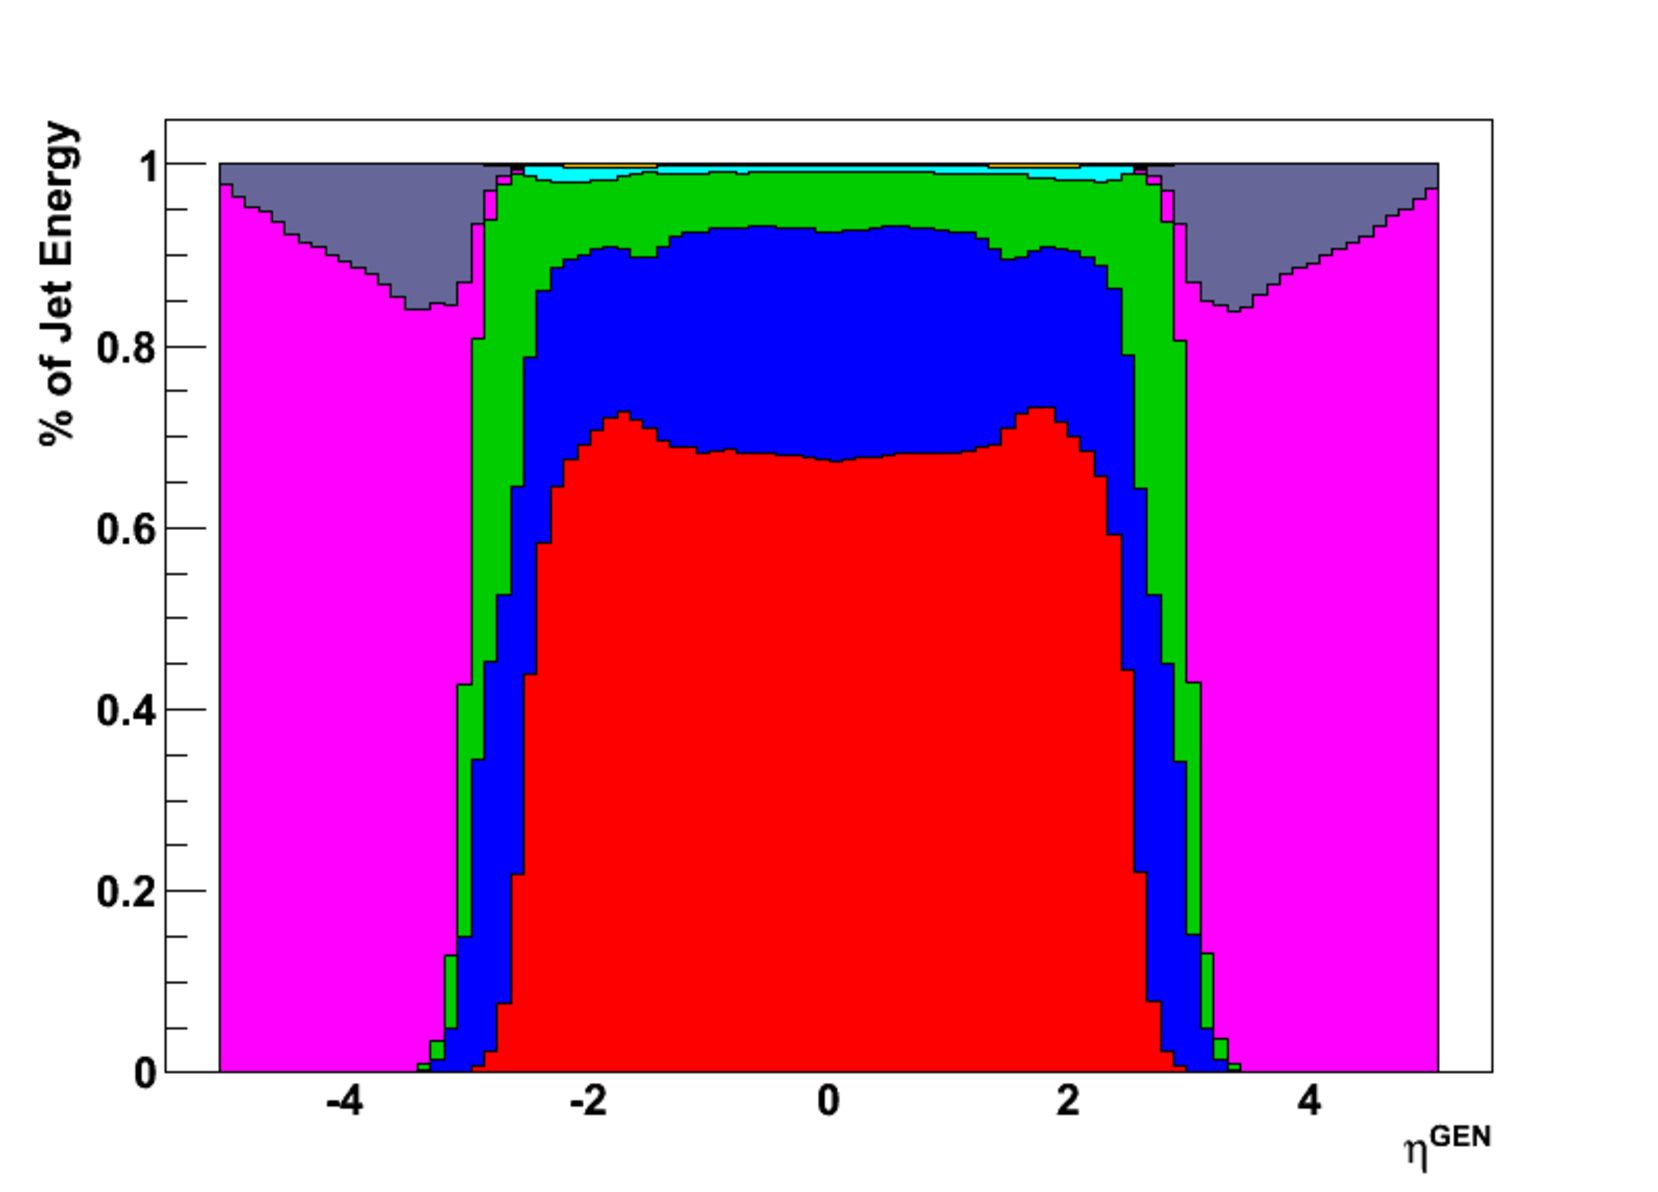
\includegraphics[width=7.5cm]{stack_R_vs_eta.pdf}}
\subfigure[]{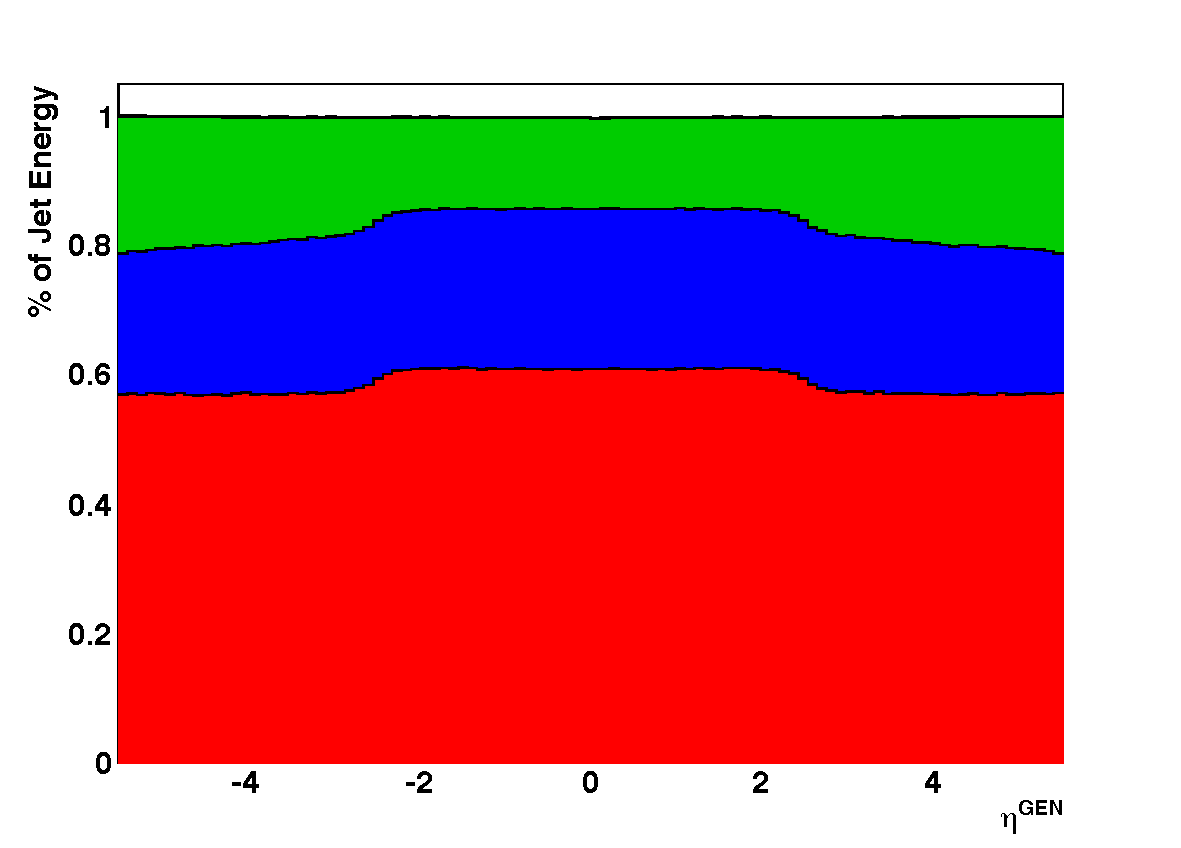
\includegraphics[width=7.5cm]{genstack_R_vs_eta.pdf}}
\caption{Average jet energy compisition as a function of generated pseudorapidity $\eta^{\mathrm{\small{GEN}}}$ for PFJets (a) and generated jets (b). From bottom to top: charged hadrons (red), photons (blue) and neutral hadrons (green), electrons (cyan). Furthermore, in the reconstructed spectrum, particles in the $3 < |\eta| < 5$ region are detected by HF and identified as hadrons (magenta) or electromagnetic particles (grey). See text for details.\label{fig:stack}}
\end{figure}

We must point out, though, that while the creation of PFCandidates is quite straightforward in the case of isolated particles (a Particle Flow photon is created from an ECAL cluster that is not ``linked'' to tracks or HCAL deposits, a Particle Flow muon when compatible hits are found in the inner tracking system and the muon chambers, and so forth), some complexities arise with bunched particles, such as the case of jets. This is because, while the CMS tracker is able to distinguish charged particles with high efficiency and excellent granularity, neutral particle detection is based on the energy deposits seen in the calorimeters, and is therefore heavily dependant on their resolutions and granularities. While this is not much of a concern for CMS's superb electromagnetic calorimeter, HCAL's inferior performance may limit the reconstruction discrimination power. 

When a reconstructed track is found to point to a calorimeter energy deposit, the Particle Flow algorithm adopts the following strategy. The sum of the momenta of the tracks $\sum p_{\mathrm{tracks}}$ is computed, and it is compared to the sum of the interested calorimetric (ECAL and HCAL) clusters $E_{\mathrm{calo}}$. If these two quantities are compatible within one standard deviation of the expected HCAL energy resolution, a Particle Flow charged hadron is created for each track, under the pion mass hypothesis. If, on the other hand, a calorimetric energy excess $E_{\mathrm{excess}}$ is observed, two cases may arise: if the excess is smaller that the total ECAL clustered energy $E_{\mathrm{ECAL}}$, a Particle Flow photon is created to account for $E_{\mathrm{excess}}$; conversely, if $E_{\mathrm{excess}} > E_{\mathrm{ECAL}}$, both a Particle Flow photon with energy equal to $E_{\mathrm{ECAL}}$ and a Particle Flow neutral hadron with energy equal to $(E_{\mathrm{excess}} - E_{\mathrm{ECAL}})$ are created.


\begin{figure}[tb]
\centering
\subfigure[]{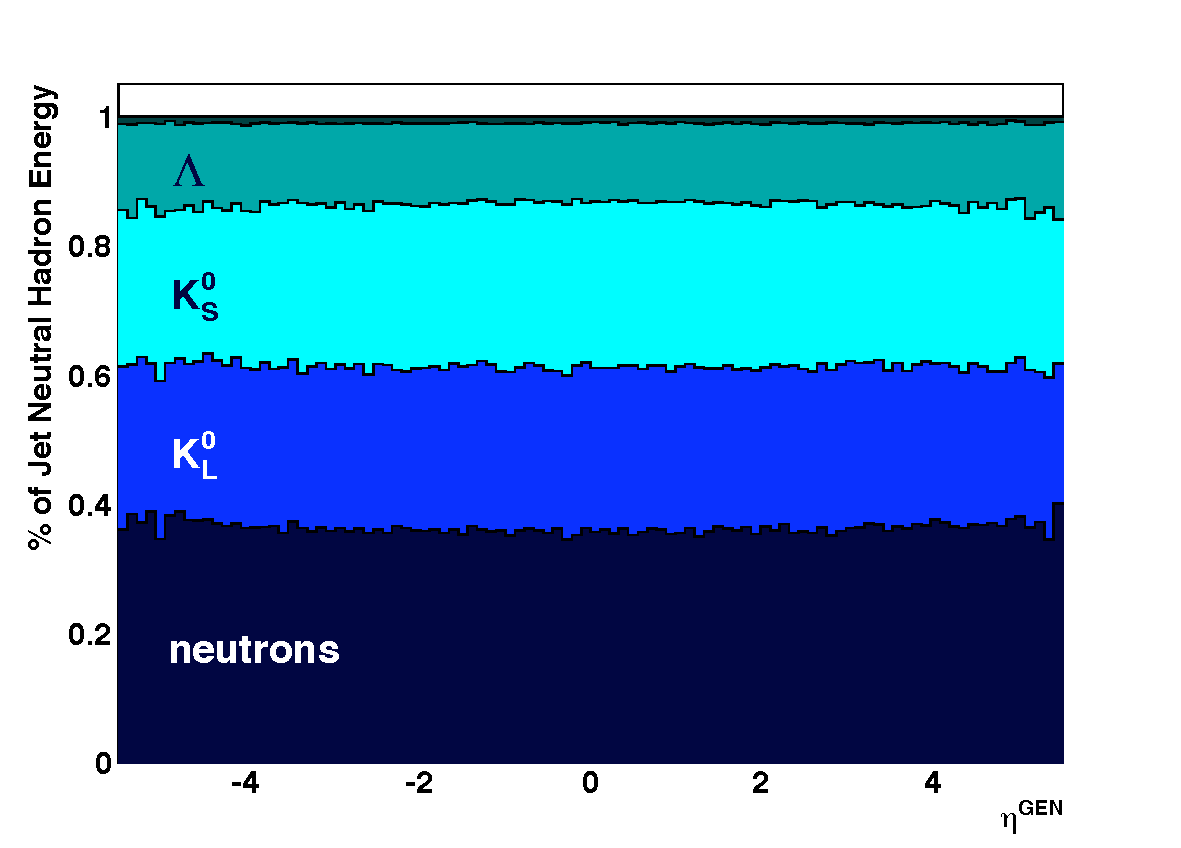
\includegraphics[width=7.5cm]{genstackNH_vs_eta.pdf}}
\subfigure[]{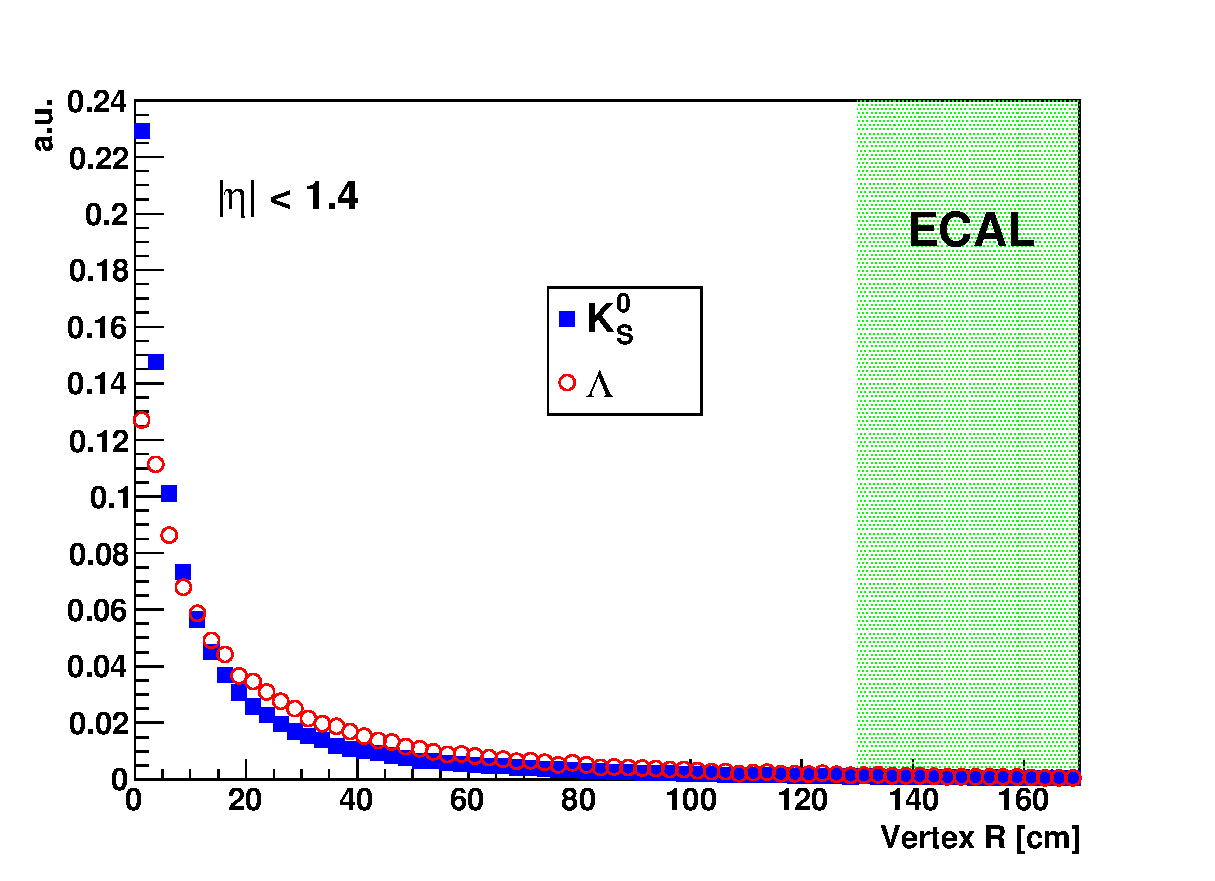
\includegraphics[width=7.5cm]{mfp.eps}}
\caption{(a): Generated jet neutral hadron energy composition, as a function of the jet pseudorapidity. From bottom to top, neutral hadron energy contributions from neutrons, $K^0_L$'s, $K^0_S$'s, $\Lambda$'s, and, on top (but not labeled on the figure), $\Xi^0$'s. (b): Distribution of the MC truth radial distance of the decay vertices for $K^0_S$ (blue squares) and $\Lambda$ (red circles) mesons produced in the barrel. The shaded band on the left shows the position of ECAL. \label{fig:stackNH}}
\end{figure}

With seven different PFCandidate types, we can introduce seven corresponding variables, that we will call respectively R$_{\mathrm{ch}}$, R$_{\mathrm{e}}$, R$_{\mu}$, R$_{\gamma}$, R$_{\mathrm{nh}}$, R$_{\mathrm{HFhad}}$ and R$_{\mathrm{HFem}}$, defined as
$$
\mathrm{R_{X}} = \frac{\sum E_{\mathrm{X}}}{E_{\mathrm{jet}}}
$$
where the sum is extended over all PFCandidates of type `X' composing the considered jet, and $E_{\mathrm{jet}}$ is the total jet energy. These variables therefore represent the fraction of jet energy that is carried by `X-type' PFCandidates.

The study of the average value of these variables as a function of pseudorapidity gives insight on the expected PFJet composition in the CMS detector. This is shown in Figure \ref{fig:stack}a, for PFJets correctly matched to generated jets, as a function of the matched generated jet's pseudorapidity ($\eta_{\mathrm{\small{GEN}}}$). Furthermore, a cut on the generated transverse momentum has been applied ($p_{\mathrm{T}}^{\small{\mathrm{GEN}}} > 80$ GeV/$c$). As expected, the charged energy fraction R$_{\mathrm{ch}}$ starts dropping in correspondance of $|\eta_{\mathrm{\small{GEN}}}|=2.5$, where the silicon tracker ends. Similarly, central calorimetry reaches up to $\eta=3$, which is where the photon and neutral hadron components start giving way to the HF components.

\begin{table} [b]
\caption{Principal decay modes and branching ratios (BR) for short-lived neutral hadrons. Values are taken from~\cite{PDG}.}
\label{tab:nhDecays}
  \begin{center}
       \begin{tabular}{ccc} \hline
      {\bf Particle} & {\bf Decay Channel} & {\bf BR} \\
      \hline
      \multirow{2}{*}{$K^0_S$} & $\pi^+ \pi^-$ & 69.2\% \\
      & $\pi^0 \pi^0$ & 30.7\% \\
      \hline
      \multirow{2}{*}{$\Lambda$} & $p$ $ \pi^-$ & 63.9\% \\
      & $n $ $\pi^0$ & 35.8\% \\
      \hline
      $ \Xi^0$ & $\Lambda$ $ \pi^0$ & 99.5\% \\
      \hline
       \end{tabular}
\end{center}
\end{table}

An equivalent jet composition spectrum can be constructed for generated jets (Figure \ref{fig:stack}b), by discriminating on the generated particles that compose these jets. In this case, though, a little delicacy is required. In fact, while classification of particles such as prompt photons and charged hadrons is quite straightforward, some complications arise in the case of neutral hadrons, for these should be classified on the basis of the actual detector reconstruction capabilities.

The average generated jet neutral hadron composition, as a function of jet pseudorapidity, is shown in Figure \ref{fig:stackNH}a. About~60\% of these particles are neutrons and $K^0_L$, which have long enough lifetimes to ensure that they reach the calorimeters without decaying. On the other hand, the remaining 40\% is composed of relatively short lived particles, which decay before reaching the calorimeters. The dominant decay channels for these particles are shown in Table \ref{tab:nhDecays}, while Figure \ref{fig:stackNH}b shows the distribution of the radial distance of the MC truth decay vertices for particles produced in the barrel ($|\eta_{\mathrm{\small{GEN}}}|<1.4$).


Neutral hadrons that decay in the CMS tracker must be classified on the basis of their decay product. Neutral pions, in particular, will rapidly decay to photons and therefore be detected in the electromagnetic calorimeter. For this reason it is correct, in the ECAL-covered pseudorapidity region, to add their energy to the photon spectrum: this explains the rise in the photon component in Figure \ref{fig:stack}b, in correspondence of the $|\eta_{\small{\mathrm{GEN}}}|<3$ region.

As for the decay to charged hadrons, the discimination is based on whether the decay vertex lies in a track seeded region of the detector or not. In the current version of the CMS software, the Particle Flow algorithm makes use of only four steps (out of five) of the CMS Iterative Tracking \cite{it_tracking}. In this implementation, track finding is guaranteed to have good efficiency even for charged particles originating from displaced secondary vertices as far as a radius of $R \approx 30$ cm deep in the transverse plane. Consequently, charged hadrons produced at $R < 30$ cm will be placed in the charged hadron component, whereas hadrons produced deeper in the detector will be kept in the neutral hadron one. For this reason the charged fraction in Fig. \ref{fig:stack}b shows a discontinuity at $|\eta| = 2.5$.

The same method has been applied to photons in jets. If a photon converts to an electron-positron pair in a track seeded region of the detector, its energy will be accounted for in the electron energy fraction. Otherwise, in the photon one.

\begin{figure}[tb]
\centering
\subfigure[]{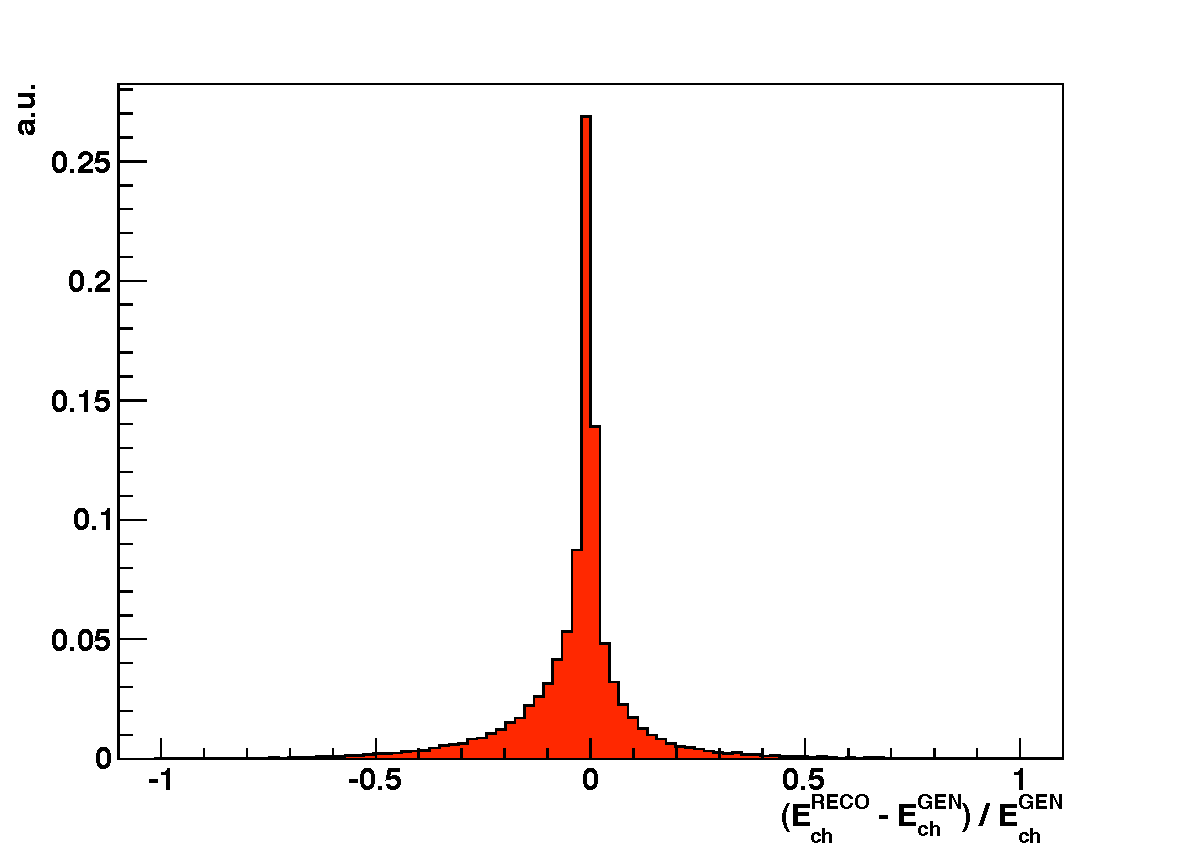
\includegraphics[width=6.5cm]{Ech_resolution_50_80_PFItCone5.pdf}}
\subfigure[]{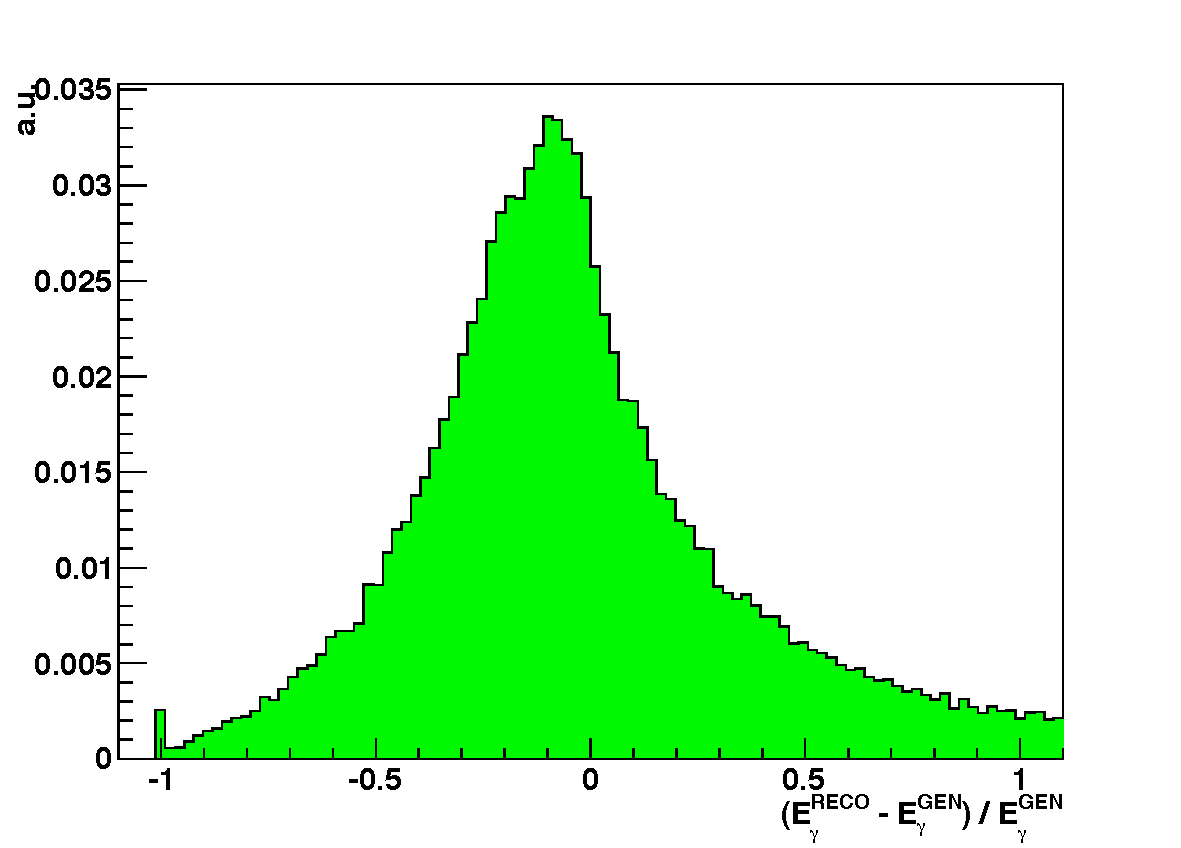
\includegraphics[width=6.5cm]{Egamma_resolution_50_80_PFItCone5.pdf}}
\subfigure[]{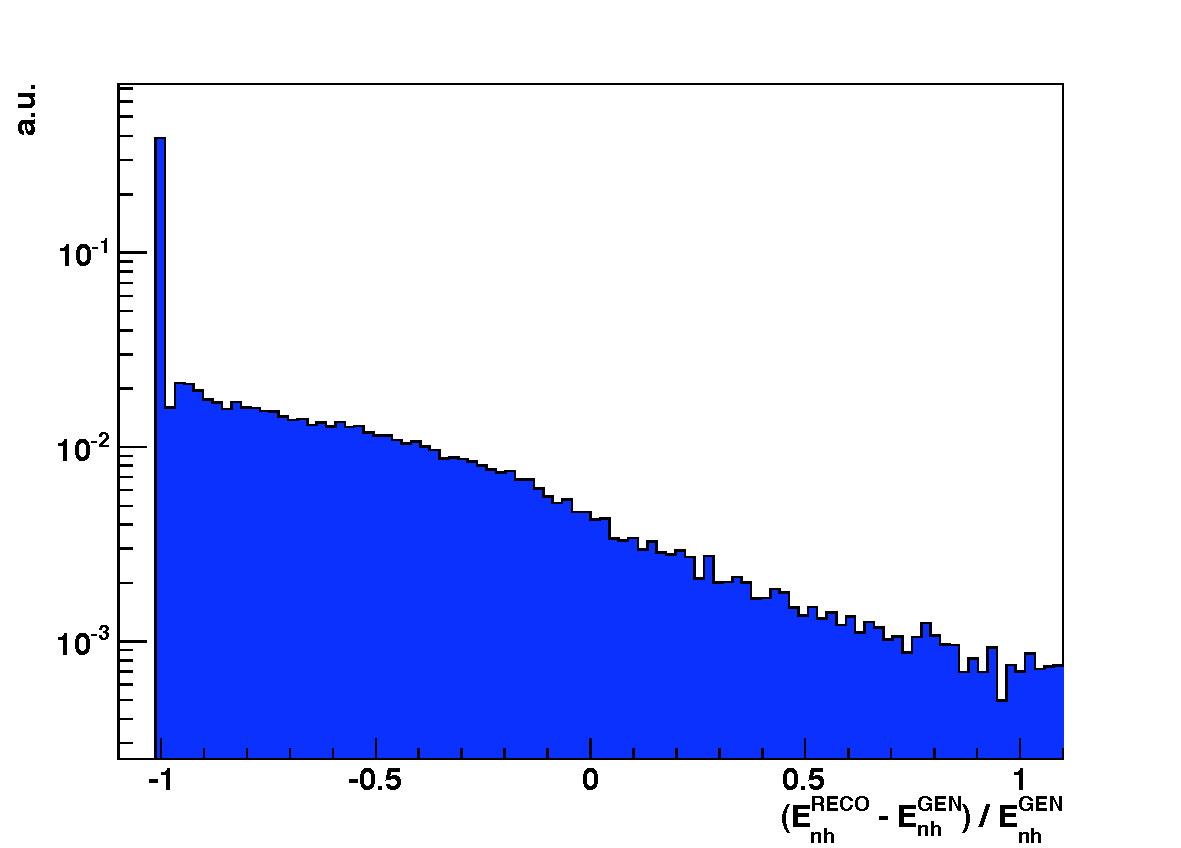
\includegraphics[width=6.5cm]{Enh_resolution_50_80_PFItCone5.pdf}}
\subfigure[]{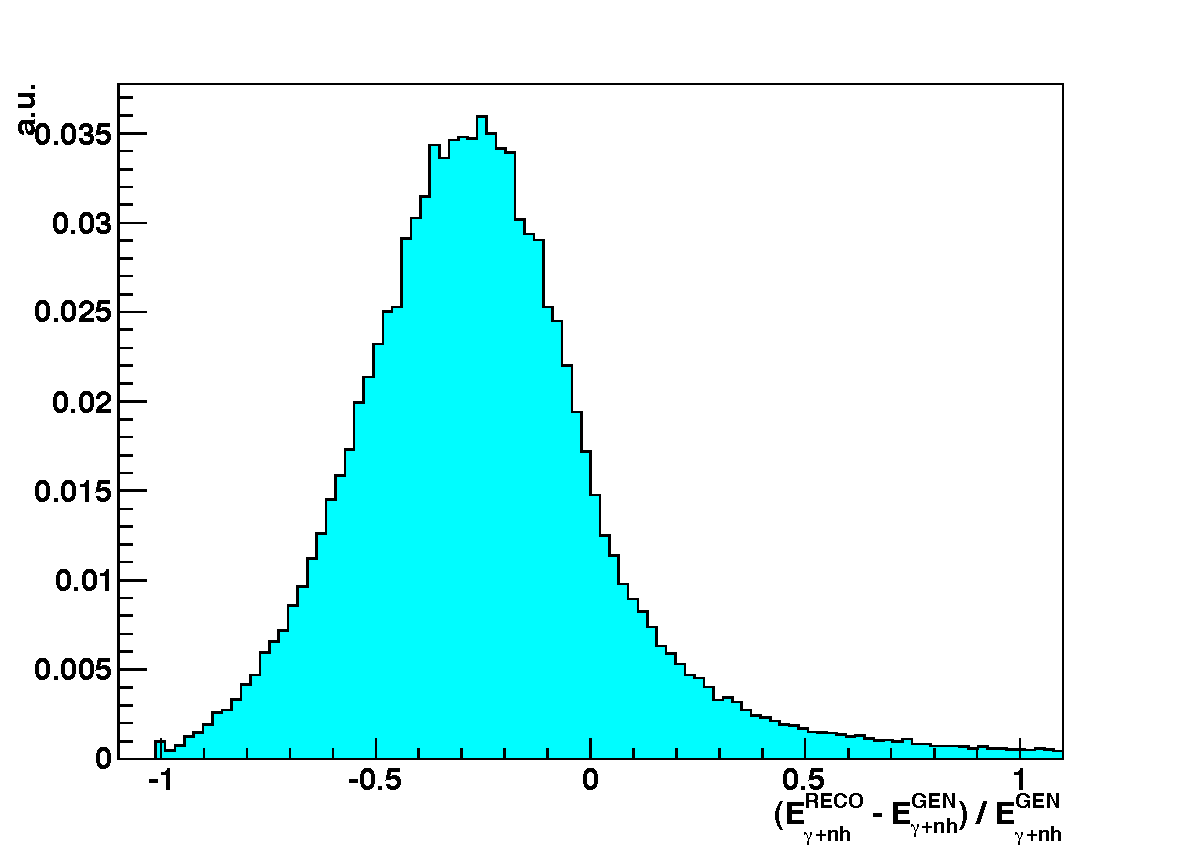
\includegraphics[width=6.5cm]{Egammanh_resolution_50_80_PFItCone5.pdf}}
\caption{Single component energy resolutions: (a) charged hadrons; (b) photons; (c) neutral hadrons; (d) photon + neutral hadron combined resolution. Distributions are normalized to unity.\label{fig:Ex_resolutions}}
\end{figure}

@@@ qui bisogna aggiornare con le figure di mikko

Figures \ref{fig:Ex_resolutions}a,b,c show, respectively, single component energy resolutions for charged hadrons, photons and neutral hadrons, for PFJets matched to generated jets that satisfy $50 < p_{\mathrm{T}}^{\small{\mathrm{GEN}}} < 80$ GeV/$c$ and $|\eta_{\mathrm{\small{GEN}}}|<2.5$. As expected, the excellent performance of the CMS tracker translates in very sharp peak in the charged energy resolution. A somewhat broader and biased distribution is obtained for the photon resolution, while for neutral hadrons an excessively large fraction of reconstructed jets (note the logarithmic scale of the $y$-axis) seem to report no neutral hadron presence, whereas the corresponding generated jets did (note the over-population of the `-1' bin).

Both the asymmetry in the photon spectrum and the anomalies in the neutral hadron one are consequence of the Particle Flow reconstruction strategy. In the case of jets, both photons and neutral hadrons, as previously described, are constructed only if a calorimetric energy excess is observed, with respect to the measured momenta of the tracks pointing to these energy deposit. For this reason it is more sound to study the {\em combined} photon and neutral hadron resolution, which is shown in Figure \ref{fig:Ex_resolutions}d. The obtained distribution is strikingly more symmetric, but has an evident bias. The amount of the bias should be directly connected to the HCAL energy resolution, on which is based the comparison that eventually gives rise to photons and neutral hadrons in jets.



\begin{figure}[tb]
\centering
\subfigure[]{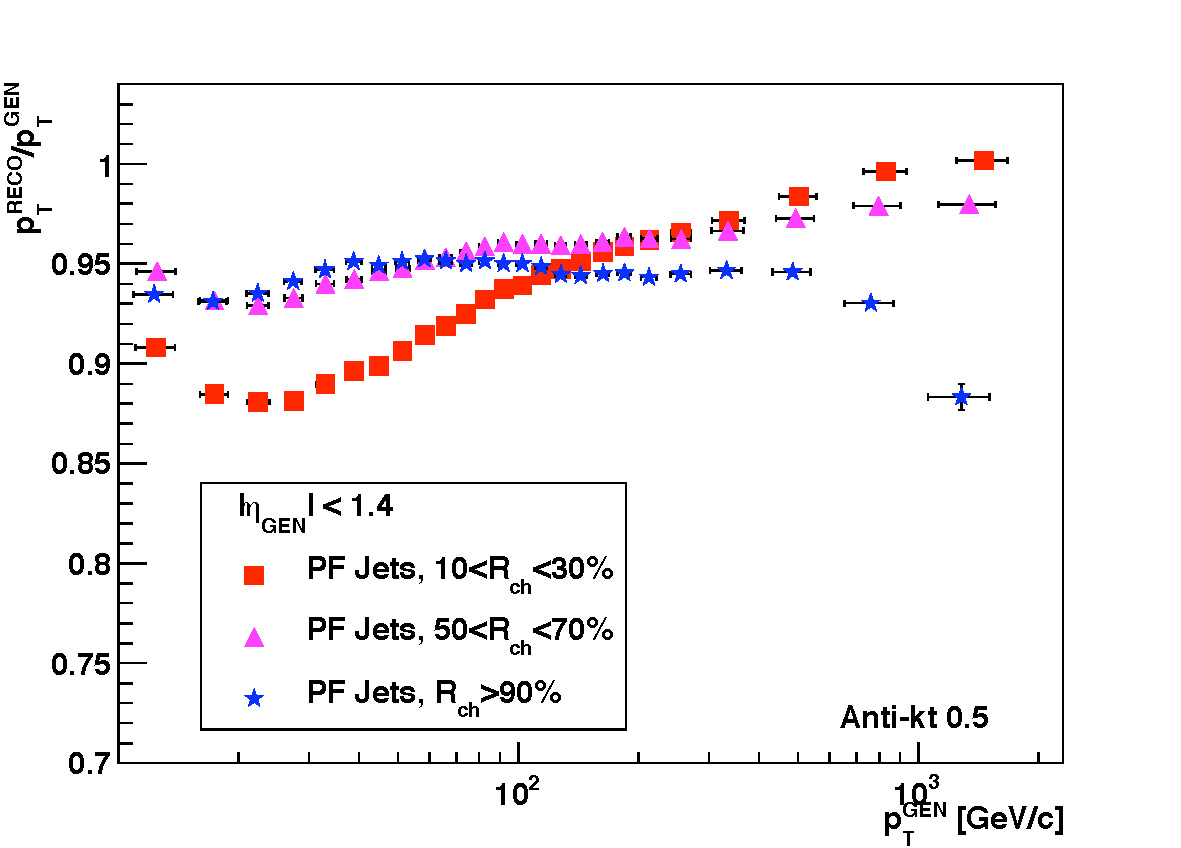
\includegraphics[width=7.5cm]{gr_Rch_response_vs_pt_MEAN_barrel.pdf}}
\subfigure[]{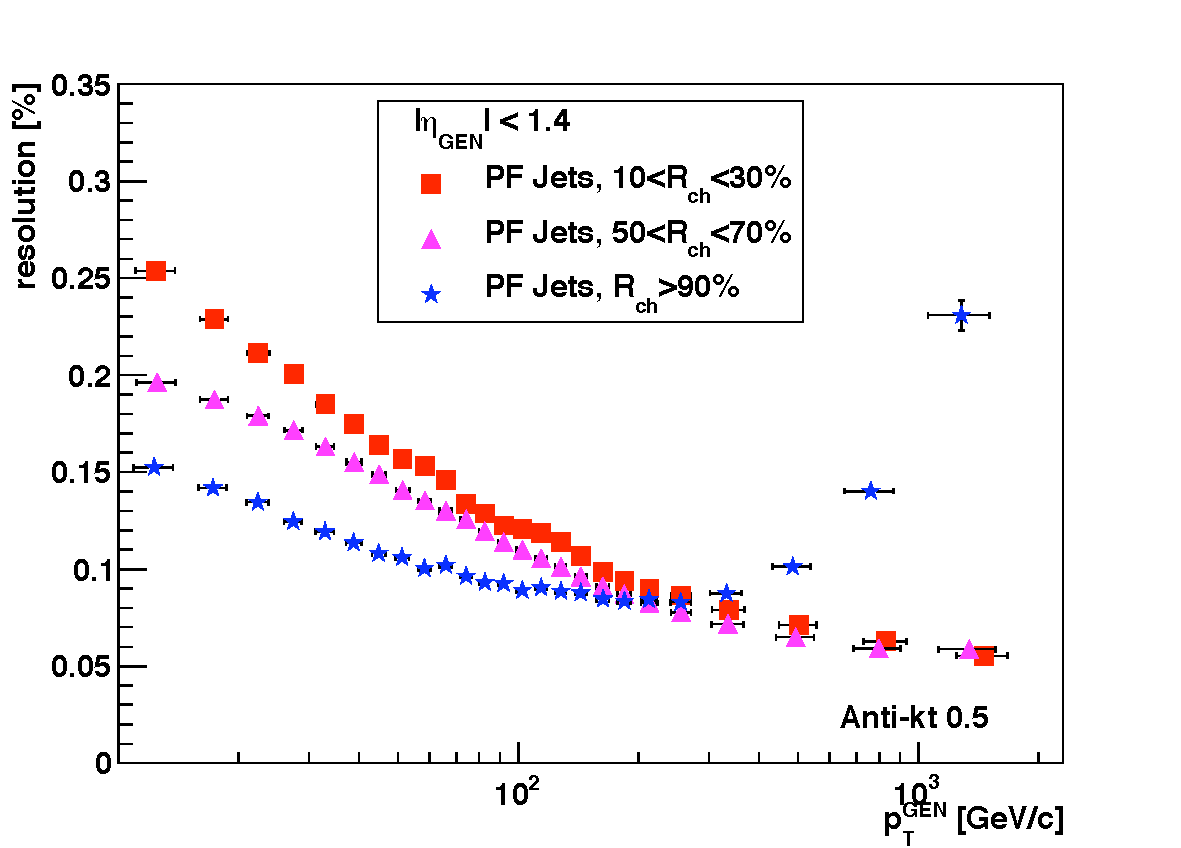
\includegraphics[width=7.5cm]{gr_Rch_resolution_vs_pt_RMS_barrel.pdf}}
\caption{Jet energy response (a) and resolution (b) as a function of the generated jet transverse momentum. The graphs compare results for PFJets and corrected calorimeter jets. \label{fig:PF_vs_calo}}
\end{figure}



\section{Response and Resolution Variation with Jet Charged Energy Fraction}
\label{sec:MCtest}

Particle Flow Jets have higher response and better resolution than calorimeter-based jets, as can be seen in Figures \ref{fig:PF_vs_calo}a,b.

\begin{figure}[tb]
\centering
\subfigure[]{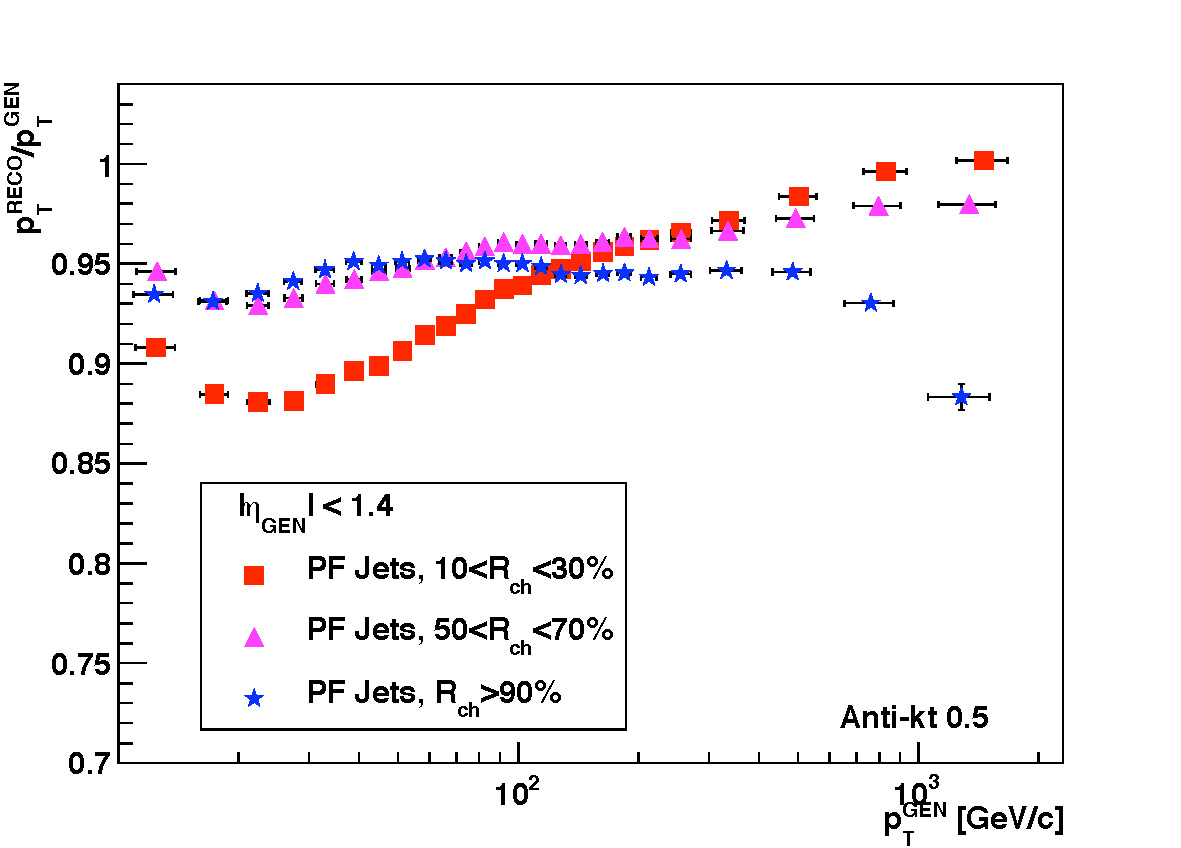
\includegraphics[width=7.5cm]{gr_Rch_response_vs_pt_MEAN_barrel.pdf}}
\subfigure[]{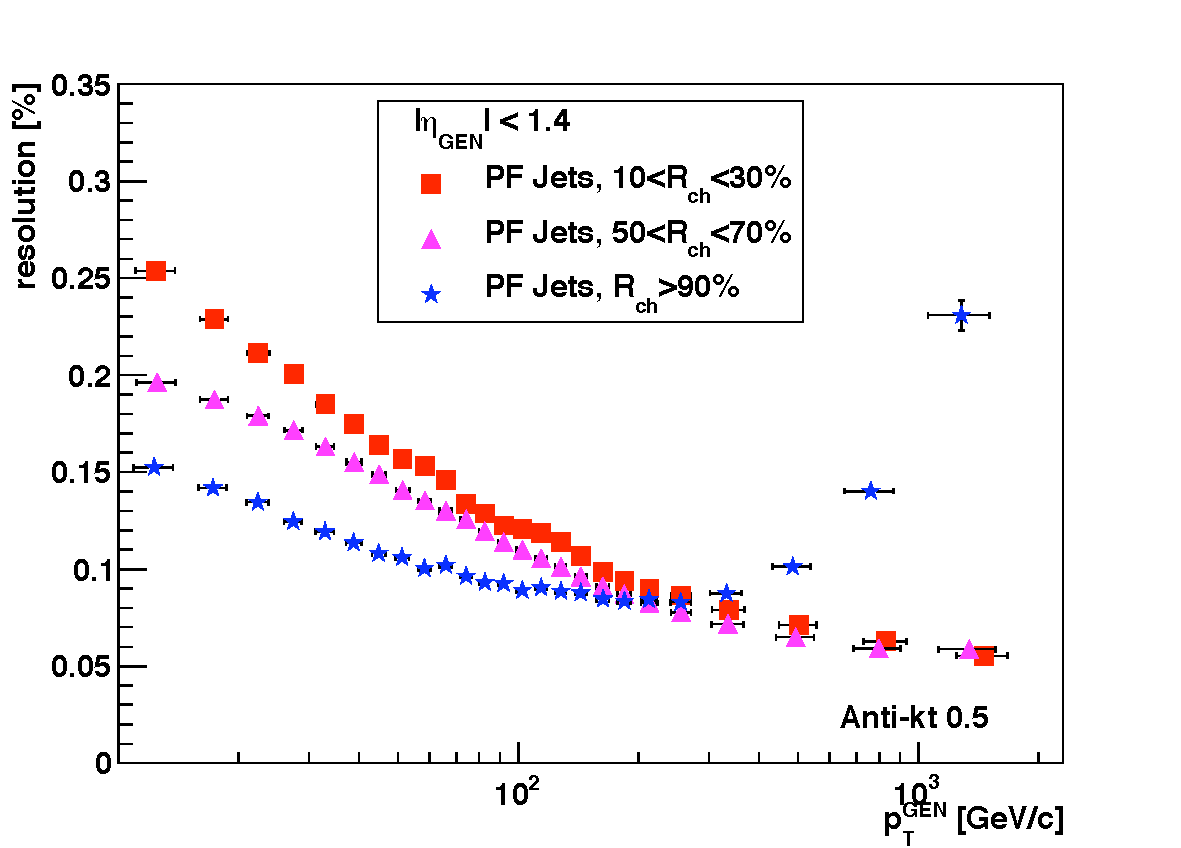
\includegraphics[width=7.5cm]{gr_Rch_resolution_vs_pt_RMS_barrel.pdf}}
\caption{PFJet energy response (a) and resolution (b) for different R$_{\mathrm{ch}}$ intervals. \label{fig:Rch_binning}}
\end{figure}

\begin{figure}[tb]
\centering
\subfigure[]{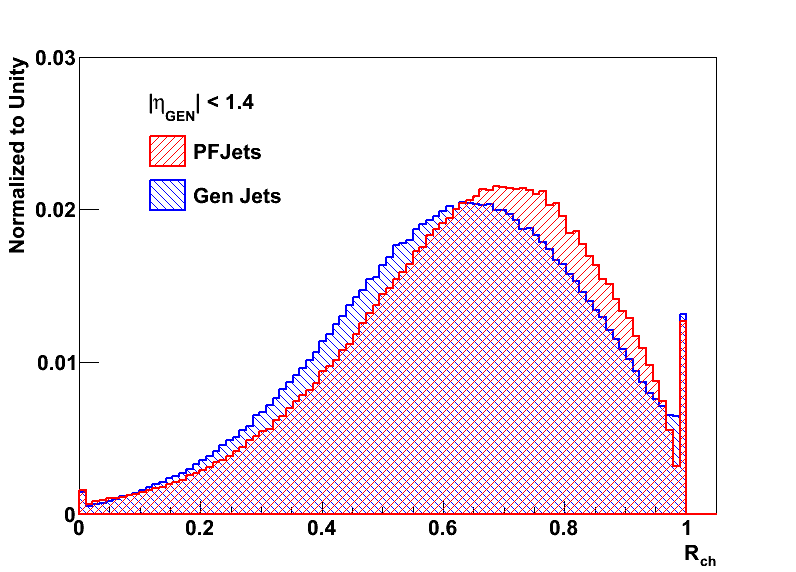
\includegraphics[width=7.5cm]{PFvsGen_Rch_barrel}}
\subfigure[]{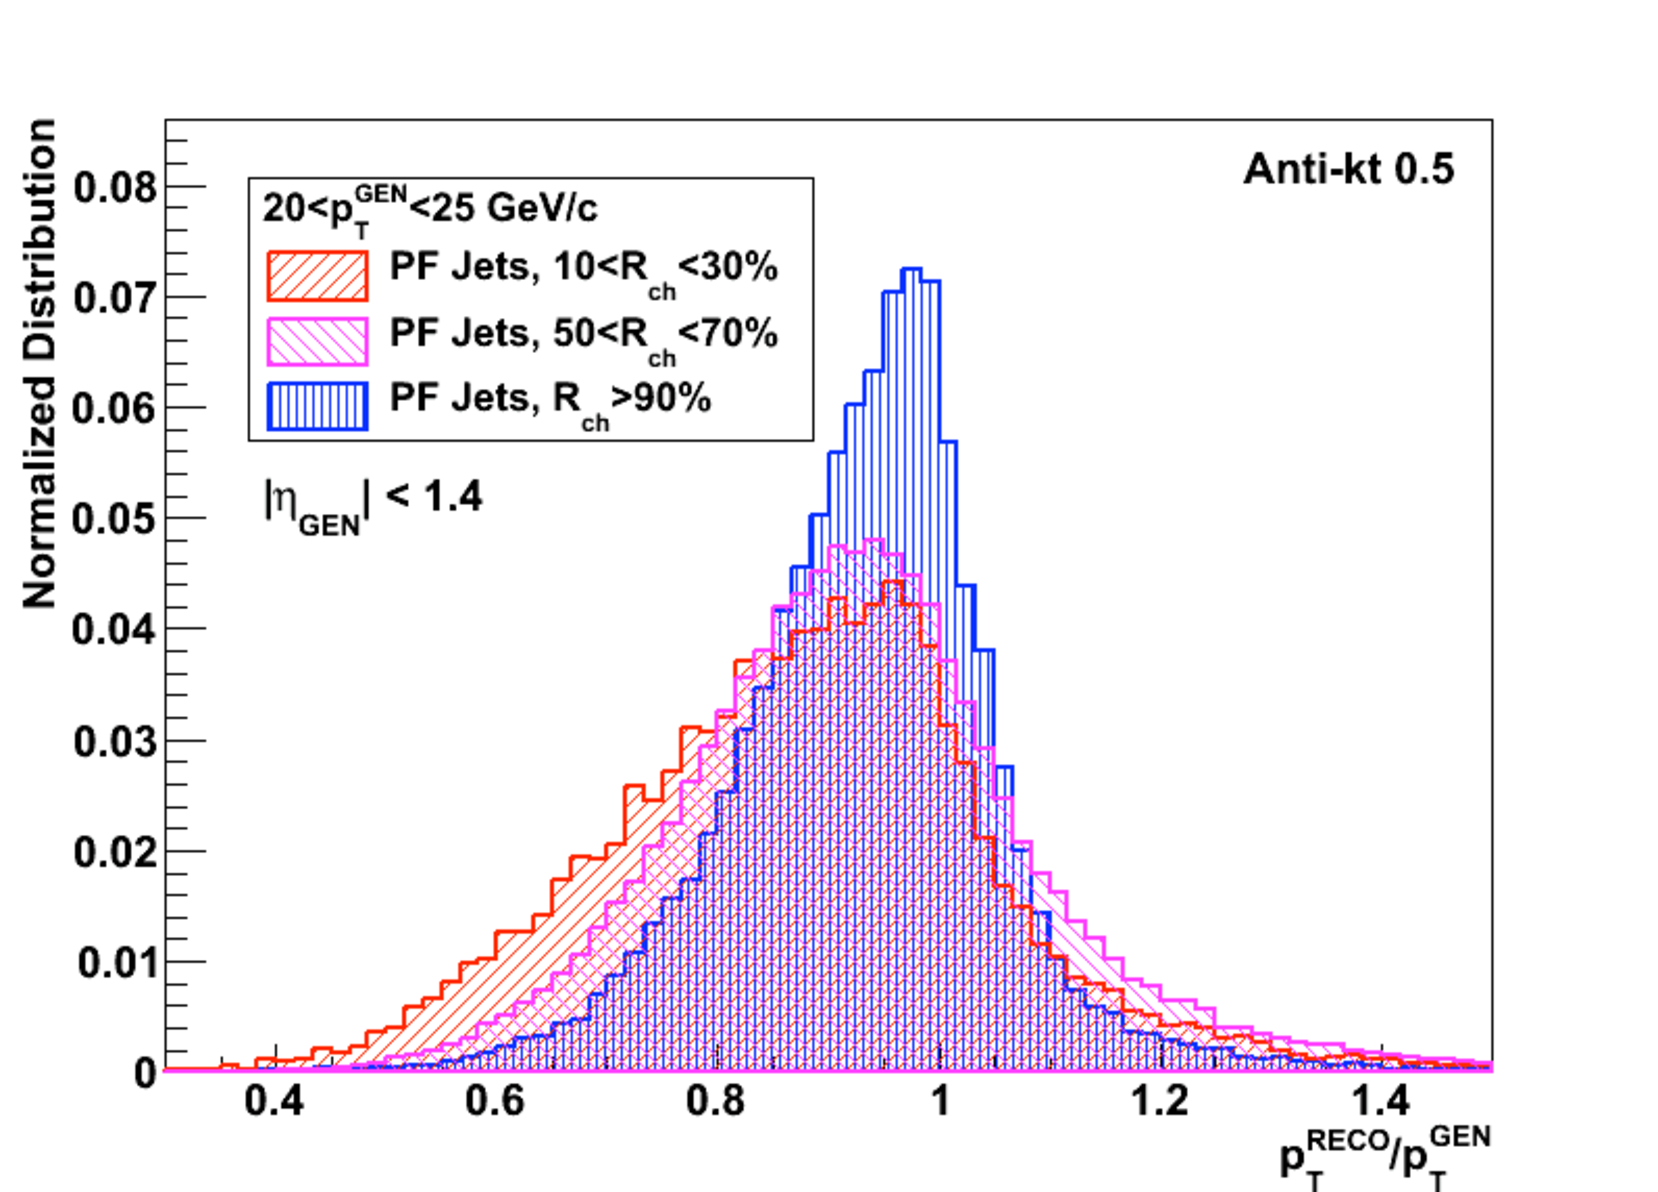
\includegraphics[width=7.5cm]{Rch_barrel_projection_3.pdf}}
\caption{(a): R$_{\mathrm{ch}}$ distributions for PFJets and generated jets in the CMS barrel, with $p_{\mathrm{T}}^{\mathrm{GEN}}>80$ GeV$/c$; (b): jet response distributions for barrel PFJets with $20 < p_{\mathrm{T}}^{\mathrm{GEN}} < 25$ GeV$/c$. \label{fig:Rch_distrib}}
\end{figure}

Therefore, if the improvement is mainly given by the use of the central tracker, it is quite straightforward to parametrize it through the variable R$_{\mathrm{ch}}$. We expect to have jets of ``higher quality'' (i.e. higher reponse and better resolution) with increasing R$_{\mathrm{ch}}$, because of a more intense use of the tracker. Figures \ref{fig:Rch_binning}a,b show jet response and resolution variations as a function of the generated jet's transverse momentum, in three R$_{\mathrm{ch}}$ intervals, for PFJets generated in the CMS barrel ($|\eta|<1.4$). For transverse momenta up to a few hundred GeV$/c$, jet quality increases with R$_{\mathrm{ch}}$, as we expected. The effect is particularly visible in the resolution graph, where at low-$p_{\mathrm{T}}$ the spread can be as large as 60\%. 

The high-$p_{\mathrm{T}}$ trend, instead, is completely inversed: at large values of R$_{\mathrm{ch}}$, jet reconstruction quality drops visibly. This behaviour is explained by two complementary reasons:
\begin{itemize}
\item track reconstruction performance worsenes proportionally to the transverse momentum of the charged particles; this effect is even more severe in the case of collinear particles;
\item the true charged fraction of a jet tends to zero as the parton momentum tends to infinity.
\end{itemize}
@@@ Qui bisogna capire cosa diavolo sta succedendo. magari presentando al PFlow e chiedendo feedback. 


Figure \ref{fig:Rch_distrib}a shows the reconstructed and generated R$_{\mathrm{ch}}$ distributions for barrel PFJets. A tranverse momentum cut of $p_{\mathrm{T}}$ has been applied on the generated jets. Figure \ref{fig:Rch_distrib}b, instead, shows jet response distributions for jets with $20<p_{\mathrm{T}}<25$ GeV/$c$, in the three studied R$_{\mathrm{ch}}$ intervals.

@@@ SMETTI DI LEGGERE QUI

Jets with increasing R$_{\mathrm{ch}}$ prove to have higher response and improved resolution, crowning this variable as a meter of the quality with which the considered jet has been measured. For the simple reason that a jet that is measured more accurately requires less (or none) energy corrections with respect to a jet that is measured poorly, we will use R$_{\mathrm{ch}}$ as a calibration variable, in such a way that these these different jet sub-populations are optimally exploited.

In order to do so, the variation of the response as a function of R$_{\mathrm{ch}}$ will be studied for each $p_{\mathrm{T}}^{\mathrm{GEN}}$ bin. The data points in each such bin are fitted with a fifth-order polinomial, and the correction is obtained as the inverse of the fitted response. Figure \ref{fig:fits}a and \ref{fig:fits}b show, respectively for barrel and endcaps, the obtained MC-truth variation for some $p_{\mathrm{T}}$ bins. The fit function is superimposed, and an overall good agreement is observed. The data points show two general trends: the first is that the response variation as a function of R$_{\mathrm{ch}}$ is more pronounced at low $p_{\mathrm{T}}$, becomes almost negligible  intermediate $p_{\mathrm{T}}$ and finally tends to invert monotony at high $p_{\mathrm{T}}$;
the second is that variations are more dramatic in the endcaps with respect to the barrel.

%The steep rise in response that is observed when R$_{\mathrm{ch}}$ approaches unity is due to a fake track infiltration, which causes an artificial rise in R$_{\mathrm{ch}}$ and, at the same time, in energy response (which may, in fact, exceed 1). It must be noted that the fake track problem has been effectively addressed in the latest release of the Particle Flow algorithm. 



As a comparison, Figures \ref{fig:genfits}a,b show the variations in MC-truth response as a function of the {\em generated} charged jet energy fraction (R$_{\mathrm{ch}}^{\small{\mathrm{GEN}}}$), in the same $p_{\mathrm{T}}$ bins. What can be observed is that while the low-R$_{\mathrm{ch}}$ behaviour seems to be compatible with the one observed in Figures \ref{fig:fits}, as R$_{\mathrm{ch}}$ grows the two sets of graphs diverge: in the barrel a very swift rise in response leads to values greater than one for jets with $p_{\mathrm{T}}  \lesssim 400$ GeV/$c$. In the endcaps, instead, all $p_{\mathrm{T}}$ bins seem to converge nicely to quasi-unitary response as R$_{\mathrm{ch}}^{\small{\mathrm{GEN}}} \rightarrow 1$, while showing opposite concavity (with respect to the reconstructed trend) at small values of R$_{\mathrm{ch}}$.



\begin{figure}[tb]
\centering
\subfigure[]{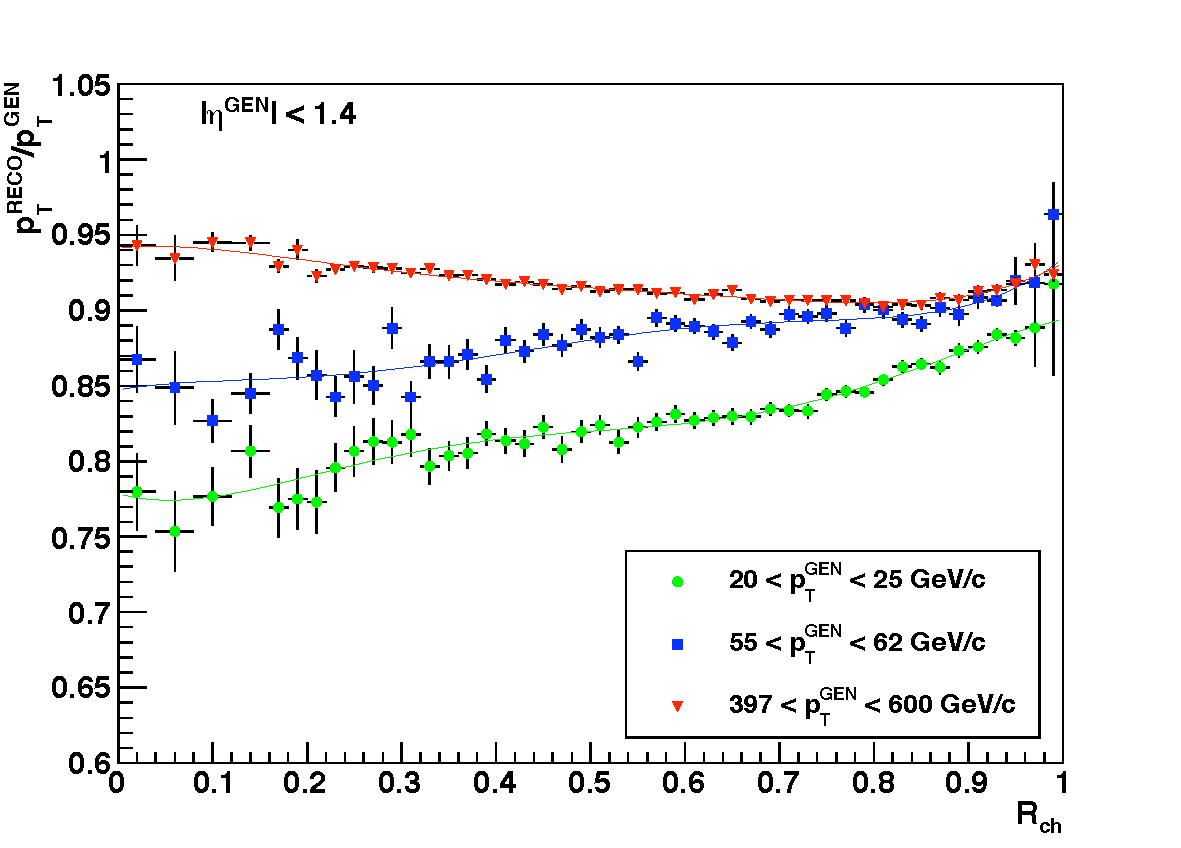
\includegraphics[width=7.5cm]{fits_barrel.pdf}}
\subfigure[]{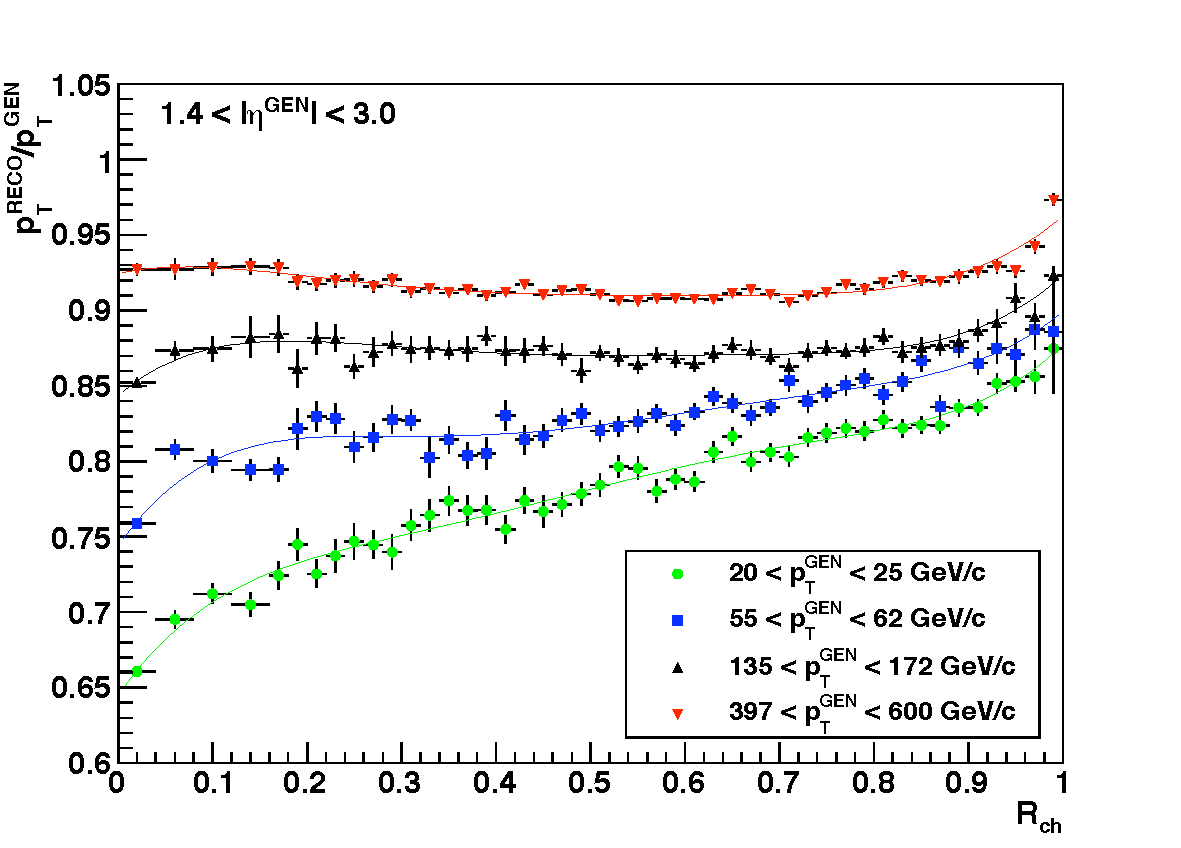
\includegraphics[width=7.5cm]{fits_endcap.pdf}}
\caption{MC truth jet energy response as a function of charged jet energy fraction R$_{\mathrm{ch}}$, for different $p_{\mathrm{T}}$ bins, in the barrel (a) and in the endcaps (b). Data points are fitted with a fifth-order polinomial. \label{fig:fits}}
\end{figure}

\begin{figure}[tb]
\centering
\subfigure[]{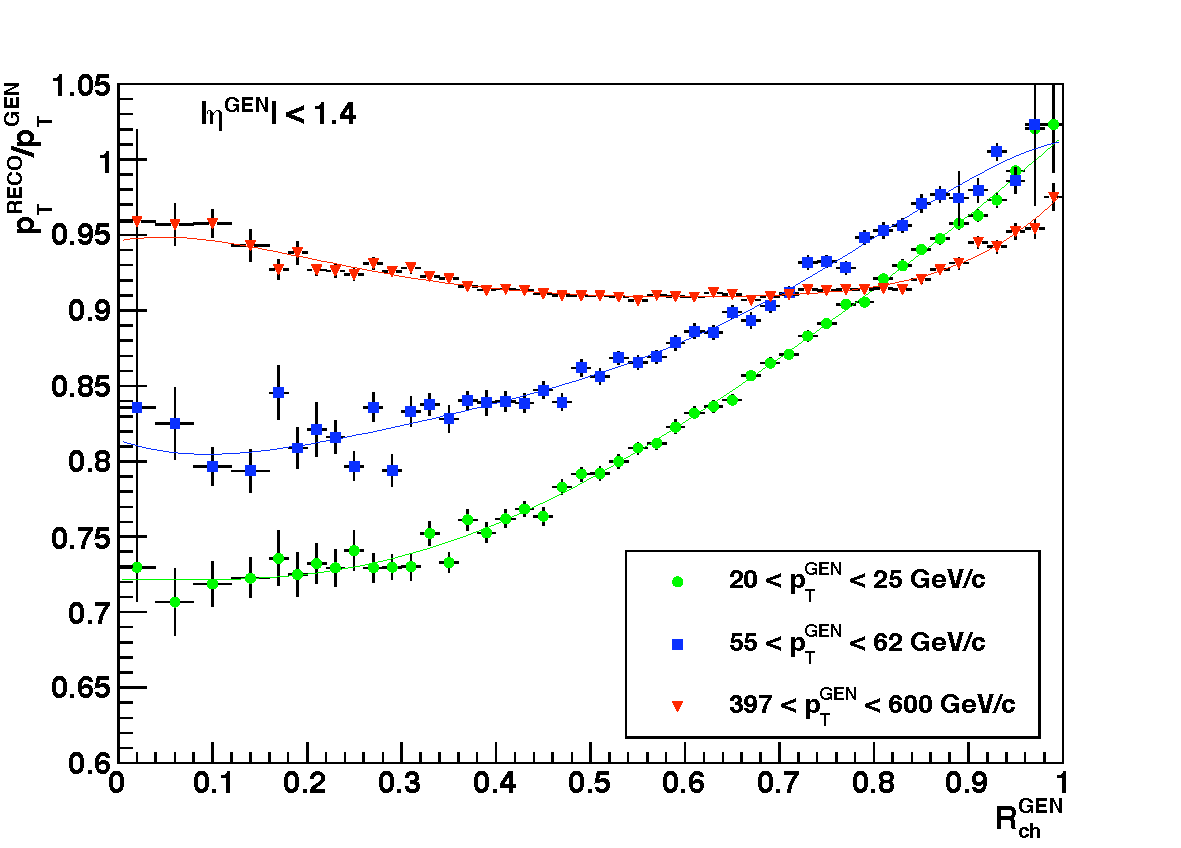
\includegraphics[width=7.5cm]{fits_genbarrel.pdf}}
\subfigure[]{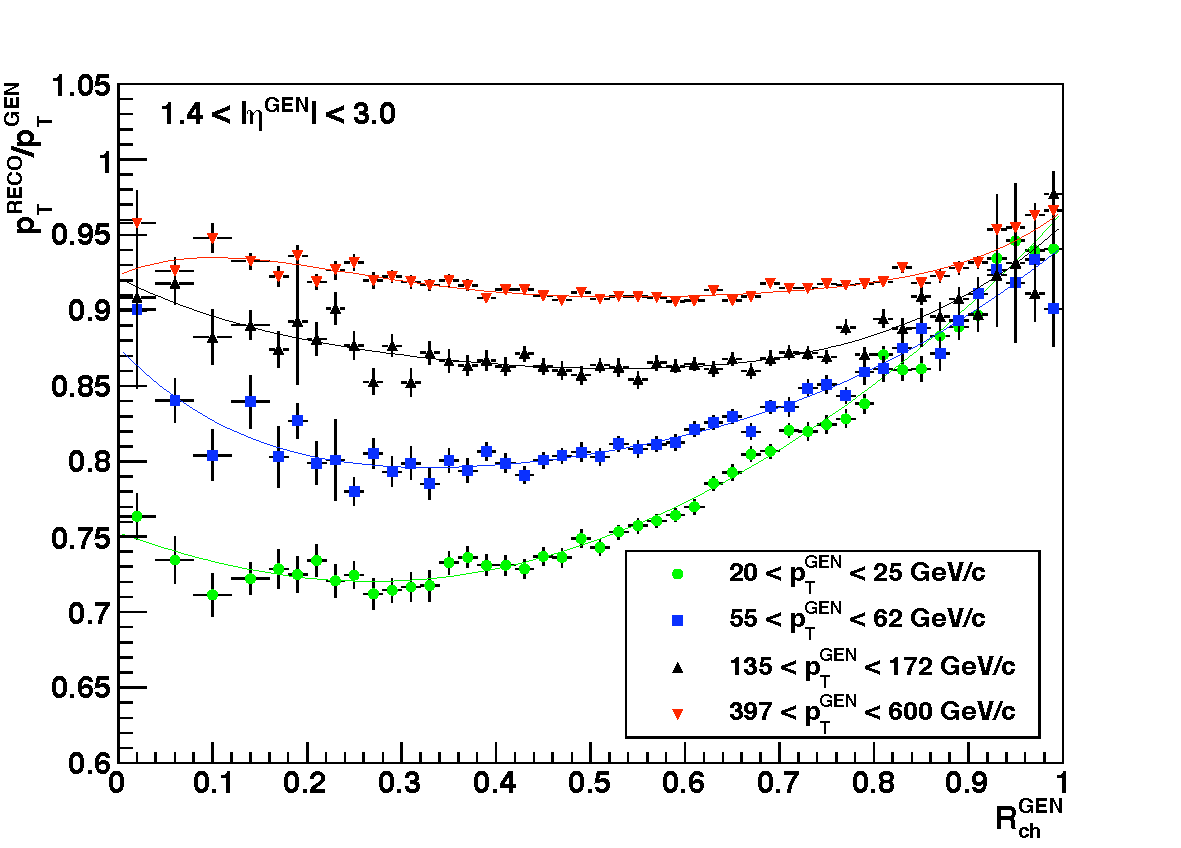
\includegraphics[width=7.5cm]{fits_genendcap.pdf}}
\caption{MC truth jet energy response as a function of the generated charged jet energy fraction R$_{\mathrm{ch}}^{\small{\mathrm{GEN}}}$, for different $p_{\mathrm{T}}$ bins, in the barrel (a) and in the endcaps (b). Data points are fitted with a fifth-order polinomial. \label{fig:genfits}}
\end{figure}



\begin{figure}[tb]
\centering
\subfigure[]{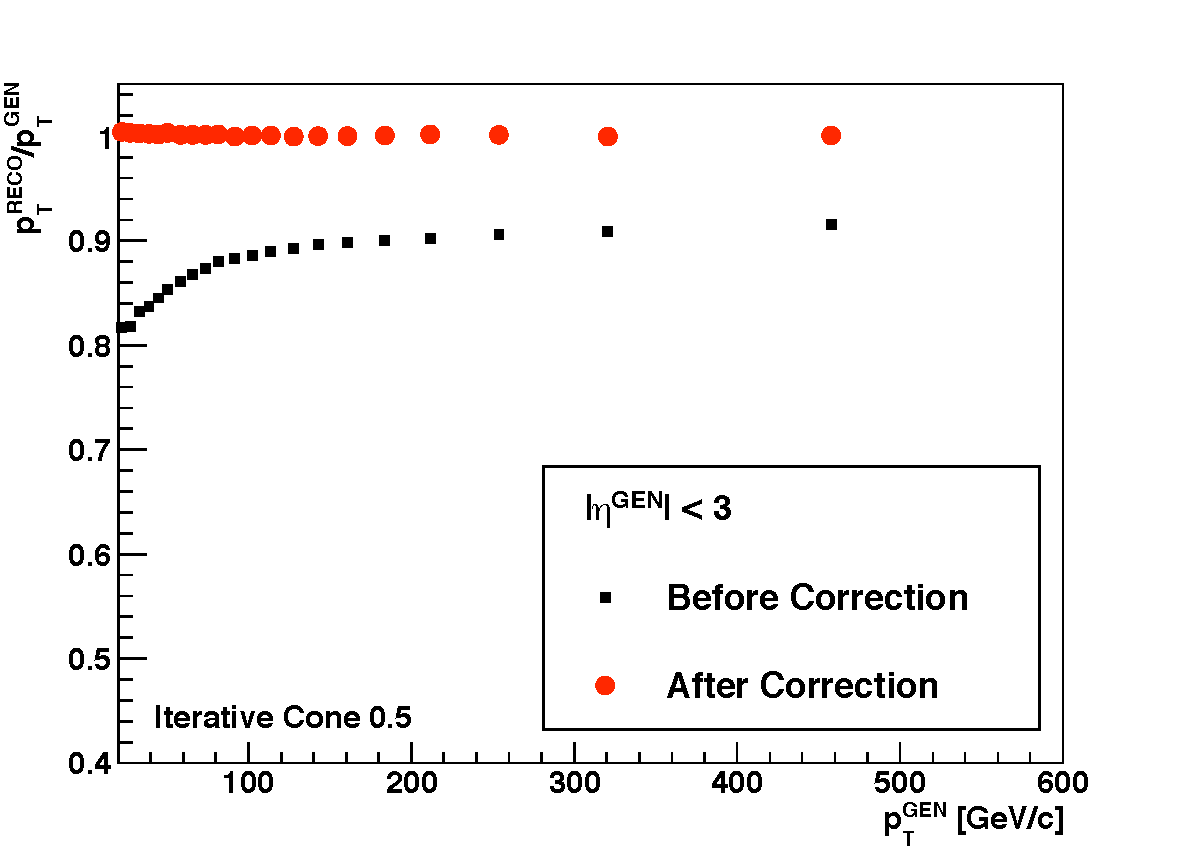
\includegraphics[width=7.5cm]{gr_Rch_response_vs_pt_MEAN_eta0_3.pdf}}
\subfigure[]{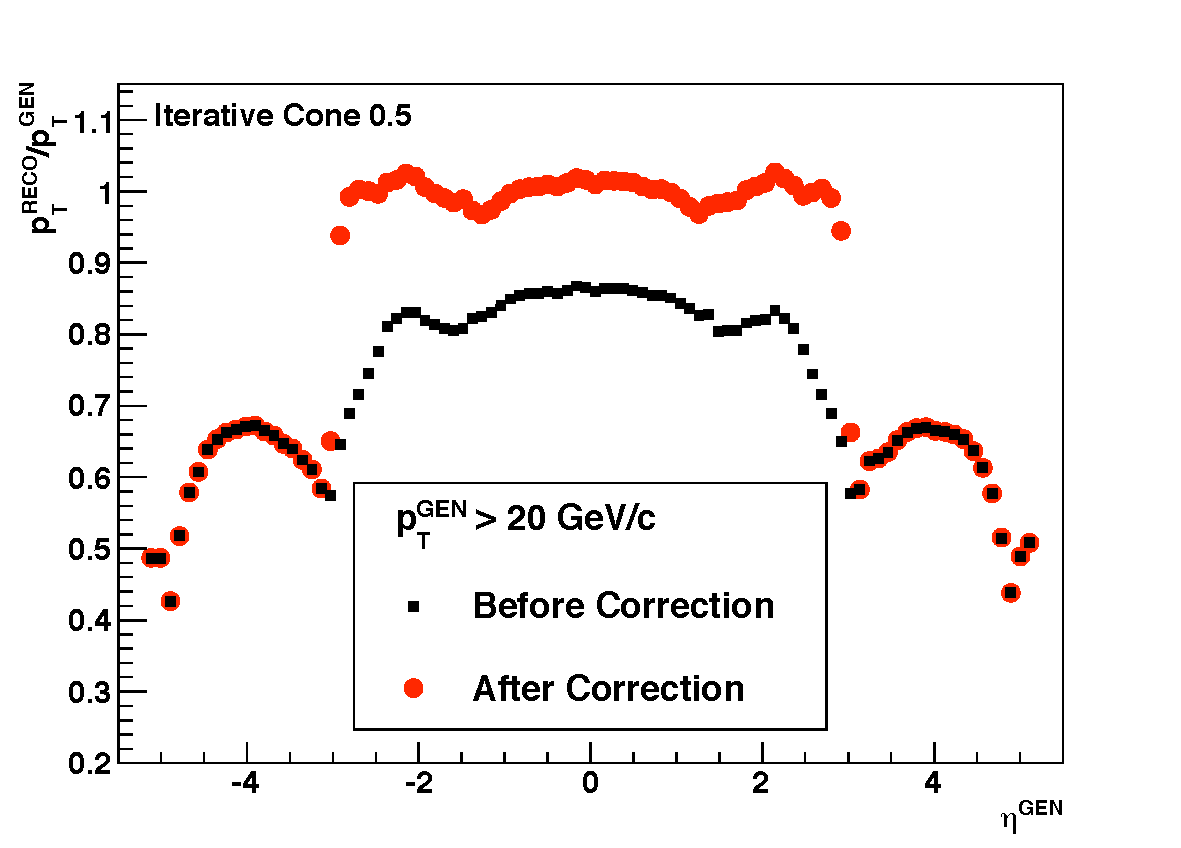
\includegraphics[width=7.5cm]{response_vs_eta.pdf}}
\caption{MC truth jet energy response as a function of generated jet transverse momentum (a) and pseudorapidity (b), before (black squares) and after (red circles) the application of the R$_{\mathrm{ch}}$-based correction. \label{fig:response}}
\end{figure}

After the corrections are obtained with the described procedure, they are applied to the same events, in order to check the method's overall consistency. Figure \ref{fig:response}a proves an effective closure test in the whole $|\eta|<3$ region by showing the obtained response as a function of $p_{\mathrm{T}}$. Figure \ref{fig:response}b, on the other hand, shows the induced variations in the pseudorapidity spectrum of the response. No artificial plateaus seem to be introduced by this correction in the $\eta$ spectrum, proving that this correction is mostly not correlated to pseudorapidity. The only exception is represented by the trackerless endcap region ($2.6 < |\eta| < 3 $), where a saturation-to-one effect seems to be introduced. This is not a concern, for the scope of this note is to quantify the maximum effect obtainable with this strategy. Furthermore, in standard jet reconstruction, PFJets will undergo the usual energy calibrations, which do include a correction as a function of pseudorapidity. This will both reduce the effect of an {\em a posteriori} R$_{\mathrm{ch}}$-based calibration, and nullify this problem.

\begin{figure}[tb]
\centering
\subfigure[]{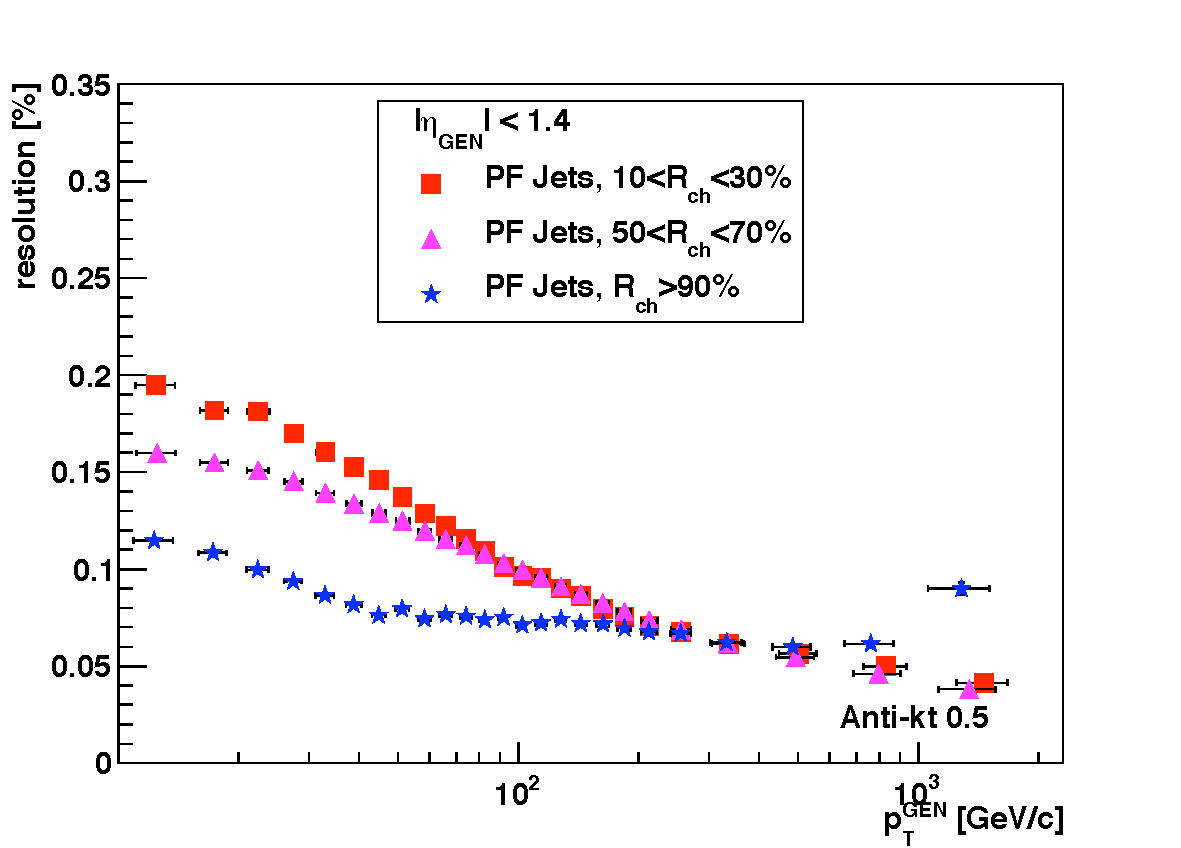
\includegraphics[width=7.5cm]{gr_Rch_resolution_vs_pt_FIT_barrel.pdf}}
\subfigure[]{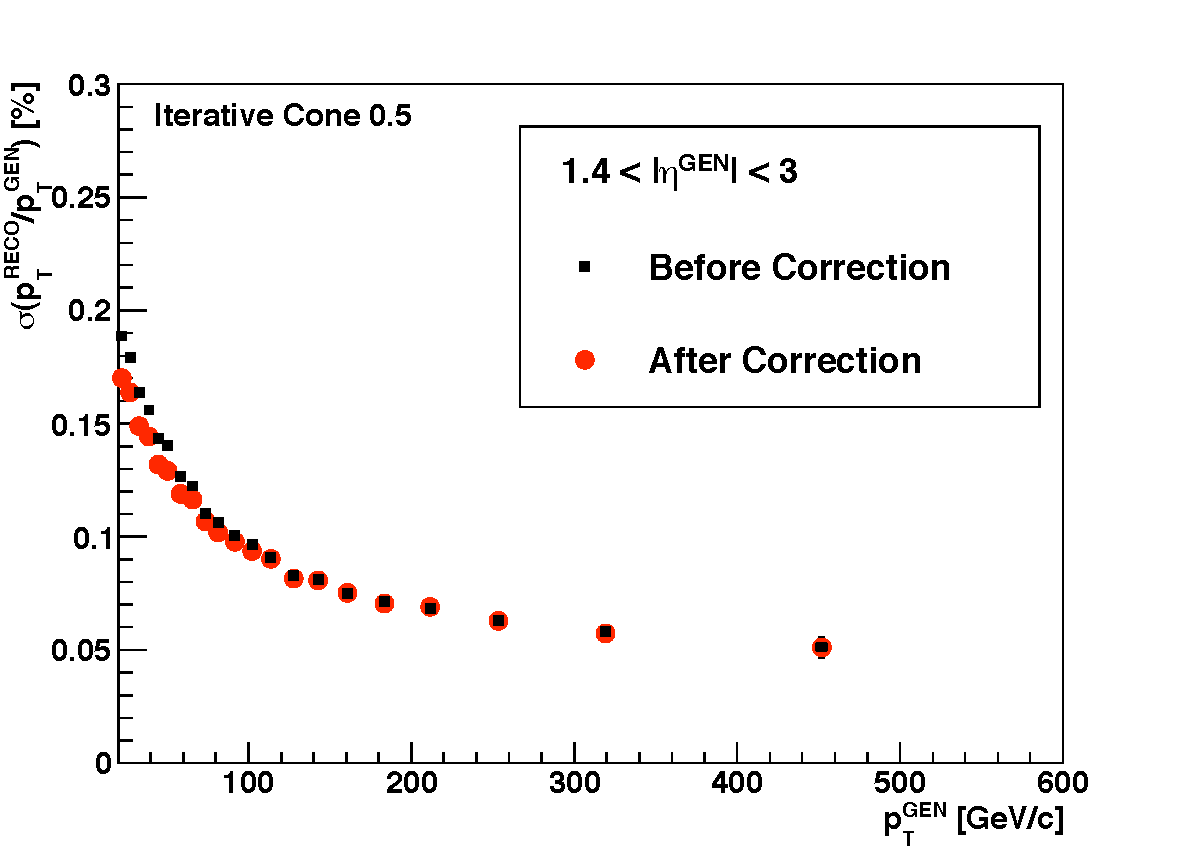
\includegraphics[width=7.5cm]{gr_Rch_resolution_vs_pt_FIT_endcap.pdf}}
\caption{MC truth jet energy resolution as a function of generated jet transverse momentum in the barrel (a) and in the endcaps (b), before (black squares) and after (red circles) the application of the R$_{\mathrm{ch}}$-based correction. \label{fig:resolution}}
\end{figure}

\begin{figure}[tb]
\centering
\subfigure[]{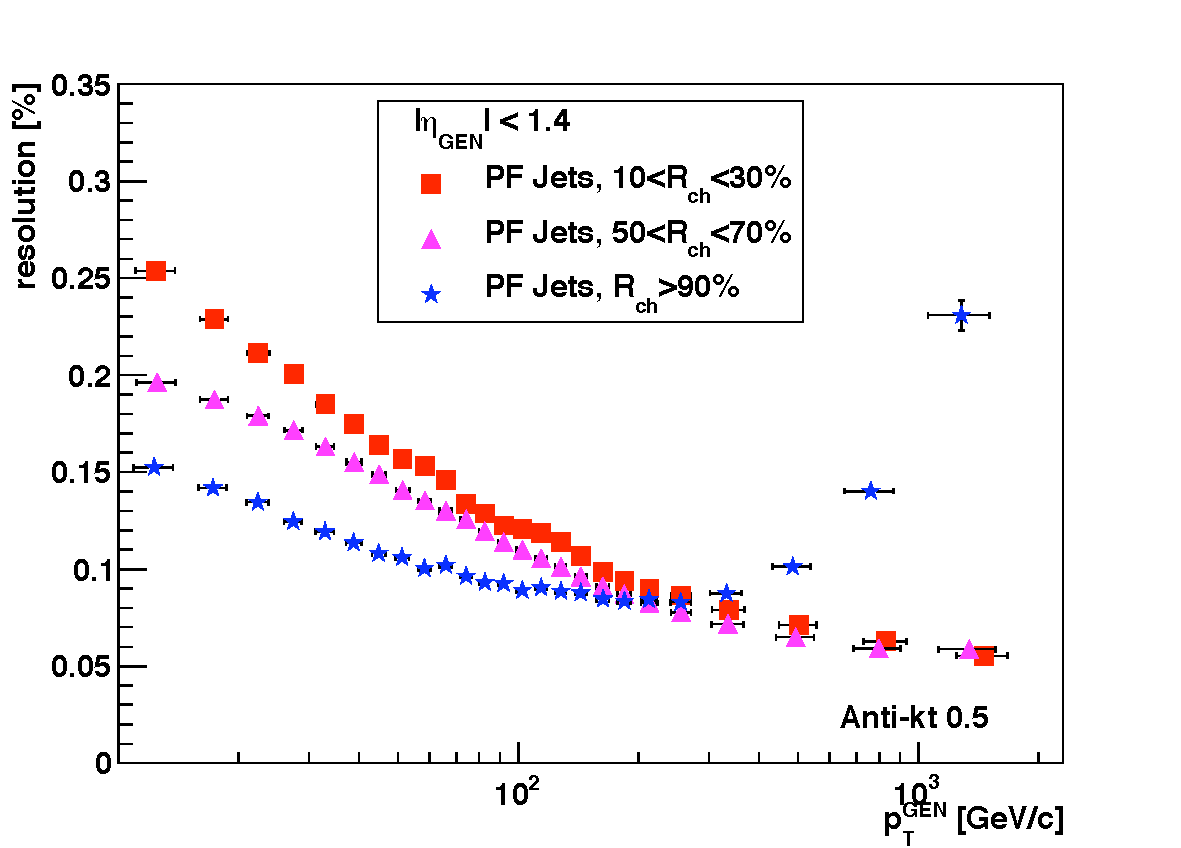
\includegraphics[width=7.5cm]{gr_Rch_resolution_vs_pt_RMS_barrel.pdf}}
\subfigure[]{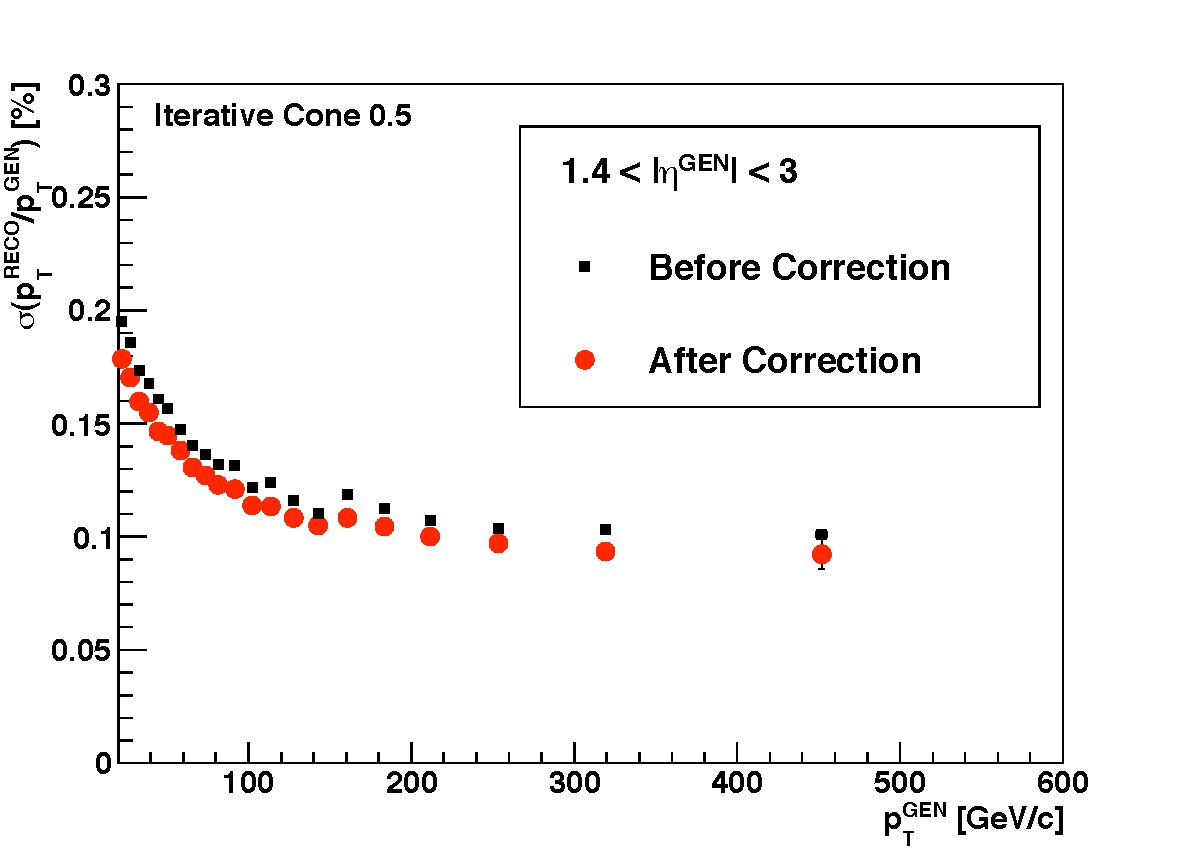
\includegraphics[width=7.5cm]{gr_Rch_resolution_vs_pt_RMS_endcap.pdf}}
\caption{MC truth jet energy resolution, computed by taking the distribution RMS, as a function of generated jet transverse momentum in the barrel (a) and in the endcaps (b), before (black squares) and after (red circles) the application of the R$_{\mathrm{ch}}$-based correction. \label{fig:resolution_RMS}}
\end{figure}

Finally, Figures \ref{fig:resolution}a and \ref{fig:resolution}b show the obtained MC-truth variation in PFJet resolution, for barrel and endcaps, when applying the R$_{\mathrm{ch}}$-based correction. Figures \ref{fig:resolution_RMS}a and \ref{fig:resolution_RMS}b, instead, show the effect induced on the resolution computed not with a gaussian fit, but by taking the distribution RMS. An overall small effect is introduced in the barrel: the improvement is of the order of 0.5\%, is localized at low $p_{\mathrm{T}}$ if considering the resolution obtained with the gaussian fit, at high $p_{\mathrm{T}}$ if considering the RMS. In the endcaps, on the other hand, a more tangible improvement is observed: it is of the order of 2\%, and localized at low $p_{\mathrm{T}}$, if considering the fit, and of the order of 1\% in the case of the RMS, but extended over the whole $p_{\mathrm{T}}$ range.
 
The following Section will focus on the construction of a data-driven method to obtain the described calibration by using photon + jet events, and comment the obtained results.







\section{Calibration with Photon+Jet Events}
\label{sec:photJet}

qui subentrate te e mikko


\subsection{Photon Identification}


\subsection{Event Selection}



\subsection{Estraction of the Correction}

e io ritorno qua: via con i plot di response vs Rch sui dati, si estraggono le correzioni, si corregge, closure test e via per la celebrita'




\section{Results}


\section{Conclusions}

\begin{thebibliography}{99}


\bibitem{pflow} {\bf CMS} Collaboration, {\em Particle-Flow Event Reconstruction in CMS and Performance with Jets, Taus and $E_{\mathrm{T}}^{\mathrm{miss}}$}, CMS PAS PFT-09/001

\bibitem{antikt} M. Cacciari, G. P. Salam and G. Soyez, {\em The anti-kt jet clustering algorithm}, JHEP 0804 (2008) 063 [arXiv:0802.1189]

\bibitem{PDG} C. Amsler et al., {\em The Review of Particle Physics}, Physics Letters {\bf B} 667 (2008)

\bibitem{it_tracking} {\bf CMS} Collaboration, {\em Track Reconstruction in the CMS tracker} (in preparation), CMS-PAS TRK-09-001~(2009)

\end{thebibliography}
%\input{intro}
%\input{samples}
%\input{selection}
%\input{trigger}
%\input{mlfit}
%\input{znn}
%\input{trackjets}
%\input{conclusion}
%%\input{appendix}
%\input{biblio}
\end{document}
